%\documentclass{../_combined/fcg-book}
\chapter{The Naming Game}

The semiotic square captures the four entities in 
a linguistic interaction: 
the {\it referent}, which is the object in the physical world that the 
speaker wants to communicate, the {\it segmented image}, which is 
the internal perception of the referent, the {\it meaning}, which is a 
category or combination of categories that picks out the 
referent in the present context, and 
the {\it utterance}, which is the word form 
or set of word forms transmitted by the speaker. In the previous 
chapters we looked at two sides of the semiotic
square. The relation between the real world and the
perceived image was studied in chapter 3 and the relation
between the perceived image and a conceptualisation that 
could act as the meaning for a language communication was 
studied in chapter 4. We now turn to the next side of 
the semiotic square: the relation between meaning and 
utterance. 

We need to find an architecture by which 
an agent can establish the relation between form and meaning, 
in other words verbalise a meaning to produce an utterance
and parse an utterance to retrieve its meaning. This 
mechanism needs to be flexible enough to deal with the 
unavoidable synonymy and amiguity that will arise. 
Second, we need to find a mechanism by which an agent 
can acquire and help construct the lexicon 
of the group. 
A shared lexicon should emerge
through the distributed activities of the agents without any prior
design or global co-ordination. Third, the lexicon formation 
process should scale up to handle a growing and ever
changing set of meanings and continue to work even with 
large populations whose constitution changes in time. 
It should be possible for new agents to enter the population
and acquire the existing language and for agents to 
leave without destabilising the whole system. These
are formidable challenges, particularly because we 
want to find the simplest possible solution, something 
a one year old child could do without fully 
developed intelligence. 

Immediately we observe a major difficulty. In realistic
language games, where agents cannot inspect each others' 
brain states nor transmit meanings directly, 
there is no feedback about the 
meaning of a word, only about the referent. For example, 
when a speaker says "wabo" and the hearer has correctly pointed 
to the referent that the speaker intended, neither the 
speaker nor the hearer can know whether they were 
using the same meaning. They can only know that they 
arrived at the same referent. When a game fails, the speaker 
can only point to the topic and the hearer then 
tries to figure out what possible meaning 
could have been applicable. The speaker cannot
communicate directly the `right' meaning, and very often more 
than one meaning is possible to distinguish a topic from 
other objects in the context, so that the hearer will 
not necessarily guess the meaning used by the speaker. 
I will call this the gavagai-problem, because Quine 
used this word to illustrate exactly this difficulty.\footnote{See \cite{Quine:1960}, p. 29,30.}
Quine evoked the problem of an anthropologist
trying to figure out what a native speaking an unknown
language might mean when he utters "gavagai" while pointing
to a white rabbit scurrying by. 

In this chapter, I will bypass the gavagai-problem by assuming
that agents get direct feedback about the meaning of a word. 
This is done by assuming that all agents share the 
same perception, that they already have
a repertoire of shared meanings, that for every agent
a particular meaning always picks out a single referent, and 
that a given referent is conceptualised with the same meaning 
by every agent. This scaffold allows us to focus on the problem
of how form-meaning associations might form and propagate in
a population without worrying how agents get feedback about 
the meanings of forms. However, it does means that we cannot 
do experiments with embodied physical agents but will have
to accept the limitation of working only
with computer simulations. 
The next chapter will take the scaffold 
away, as any serious theory for word meaning 
acquisition should. I will then show that given an 
appropriate coupling between lexicalisation and categorization, 
a communication system can still get off the ground based on 
the mechanisms described in this chapter. 

\section{Inventing a lexicon}

\is{Naming Game}I will now introduce another game, the Naming
Game, to allow us to focus on the origin of the lexicon.
The Naming Game defines a situation requiring 
a group of distributed autonomous agents to develop and 
use a shared lexicon relating forms and meanings, 
assuming they have a shared repertoire of meanings and get 
direct feedback about what meaning corresponds to a
certain form. The Naming Game can be thought of 
as the lexical side of the Guessing Game.\footnote{
The Naming Game and associated computer simulations
were presented for the first time in \cite{Steels:1996a}.}
The game can be implemented with different
mechanisms compared to the ones I will use, so it defines a 
task setting in which different solutions can be compared. 
See also \cite{Hutchins:1995}.
A different task setting for studying language acquisition
(but not how a language may emerge from scratch) is 
illustrated in \cite{Regier:1996}. In this case, the agents
are shown examples and counter-examples together with 
words they should use in each case. 
\newline 
It can be objected
that the Naming Game (and the Guessing Game) already 
assumes that the agents want to communicate. 
This is true, but the game can be embedded in a larger
setting where communication is vital for survival. 
An example of such a setting is discussed in \cite{Werner:1991}. \newline
Another issue concerns
the evolution of the game itself. This topic is discussed in: 
\cite{Hurford:1989}. This paper is also
the earliest paper posing the problem of the origins of 
a lexicon through computational simulations. See also: 
\cite{Oliphant:1996}. \cite{Hauser:1996}
contains a further discussion of these topics from the 
viewpoint of biological continuity.

The Naming Game is played by two agents, a speaker and 
a hearer, which are picked randomly from a population. 
The speaker selects a meaning from the shared repertoire
of meanings, looks up a possible word for this meaning 
in his lexicon, and transmits the word to the hearer. 
The hearer interprets the word by looking it up in his lexicon, 
and transmits the meaning he thus obtained. If this meaning 
is the one that the speaker originally had in mind the 
game succeeds, otherwise the game fails. When the game 
fails, the speaker communicates the meaning directly so 
that the hearer can acquire a new form-meaning pair 
for later conversations. When a speaker does not have a
word yet for a meaning he wants to communicate, he may create 
a new one. 

\subsection{Representing lexical associations}

What cognitive architecture do agents need to engage in naming 
games? Clearly they need some sort of {\it associative memory} to\is{lexical memory}
store their individual lexicons.
Let us assume that agents 
can construct and recognise arbitrary consonant-vowel combinations, 
like "coba" or "wabidu", for forming words, and that they 
have a repertoire of possible meanings in the form of 
categories, for example [LEFT], [DARK], [LARGE], etc. 
The contents of the associative memory of a single agent can
be displayed in a table as follows: 
\begin{table}
\begin{center}
\begin{tabular}{ l  l }
\lsptoprule
{\it meaning} & {\it form} \\ \midrule
[DARK] & coba \\ \midrule
[LARGE] & wabidu \\ \midrule
... & ... \\ \midrule
\lspbottomrule
\end{tabular}
\end{center}
\caption{\label{tab:t-mem} Associative memory of a single agent.}
\end{table}
As an agent is acquiring his lexicon, there are going to 
be stages when he is not yet sure about the meaning of 
a certain form. So it must be possible for the agent
to store different 
meanings for the same form and different forms for the
same meaning. This can easily be done by extending the memory capacity
to cross-associate multiple items. Agents can then 
handle amiguity (one word can have different
meanings) and synonymy (one meaning can 
be associated with many different words). 

A speaker can only transmit a single choice for 
expressing the meaning.
When there are alternative words for the same meaning in 
his lexicon, he must decide which one to use and this decision
should be such that it maximises success in the game. 
To estimate this success, 
each agent should monitor for each form-meaning association
how successful it has been, which could be implemented 
by associating with every form-meaning pair 
a {\it score}.\is{score} The score of a form-meaning pair
is specific to an agent and based only on his own 
local interactions with other agents, in line with the 
principle that no single agent has a complete overview of 
the lexicon nor controls the others. An example of 
a lexicon with multiple associations and a score for every 
association is illustrated in \tabref{tab:mem2}. 
\begin{table}
\begin{center}
\begin{tabular}{c c c c  c  c  c } \midrule 
& coba & zapo & bila & pama & wabidu & limiri \\ \midrule 
[DARK] & 0.3 & 0.2 & 0.1 & 0.8 & - & - \\ \midrule
[LARGE] & - & - & - & 0.5 & 0.3 & 0.6 \\ \midrule
\lspbottomrule
\end{tabular}
\caption{\label{tab:mem2} Example lexicon with multiple associations.}
\end{center}
\end{table}
From this table we see that the agent prefers to use the 
word "pama" for [DARK] and "limiri" for [LARGE]. 

\subsection{Updating the score}

One of the crucial aspects of the Naming Game model
is how scores are updated based on the outcome of 
a game. Intuitively 
the score should be related to use and success. 
The more a word is used and the more success it 
has, the higher the score should be. Moreover
there should be a time dimension, 
as recent use and success should obviously contribute
more to the current score. 
The following is a scheme that captures these
characteristics. 

Every time an agent successfully uses a form-meaning pair 
for speaking, he increments
the score with a specific increment $\delta$. 
$\delta$ is relatively high, typically equal to 0.1. 
The scores of competing associations, i.e. 
associations that used another form for the same meaning
are decremented with $\delta$. The score remains however bounded 
between 0.0 and 1.0. This way the `best' 
form-meaning pair stands out more clearly next time 
around.\footnote{A systematic investigation of alternatives for 
the updating function is contained in \cite{Oliphant:1997}. 
The dynamics of the mechanisms used in the 
Talking Heads experiments are being investigated in the
Ph.D thesis of Frederic Kaplan.}

When an agent plays the role of hearer, he also increments
the association that was successful with $\delta$, and 
decrements competing associations, i.e. associations that related
another meaning to the same form. When a 
game fails, the associations used by the speaker
and the hearer that contained the transmitted 
word form are both decremented. 

The operations of speaker and hearer are summarised in 
\figref{incr-decr} assuming that speaker and hearer
use both the score table above (in reality they of 
course always have different score tables). 
The speaker collects all possible
forms for a given meaning [DARK], chooses the one with the
highest score ("pama"), and transmits that form. 
The hearer collects all possible meanings for 
the transmitted form ([DARK], [LARGE]) and again chooses the one with
the highest score. If the hearer's meaning is equal to that
of the speaker's, the game succeeds. The score of 
two used associations increases and the others
decrease, implementing lateral 
inhibition. If the game fails, only the two used associations 
go down.\footnote{More or less neural realism can be introduced to 
model this associative memory. In our experiments we 
have a perfectly working memory that can store an 
association as soon as it has seen it once. This makes
theoretical investigation easier and makes it possible
to better follow the simulations and experimentations.  
An example of a neural network solution to lexical
memory is discussed in \cite{Cangelosi:1996}.}

\begin{figure}[htbp]
  \centerline{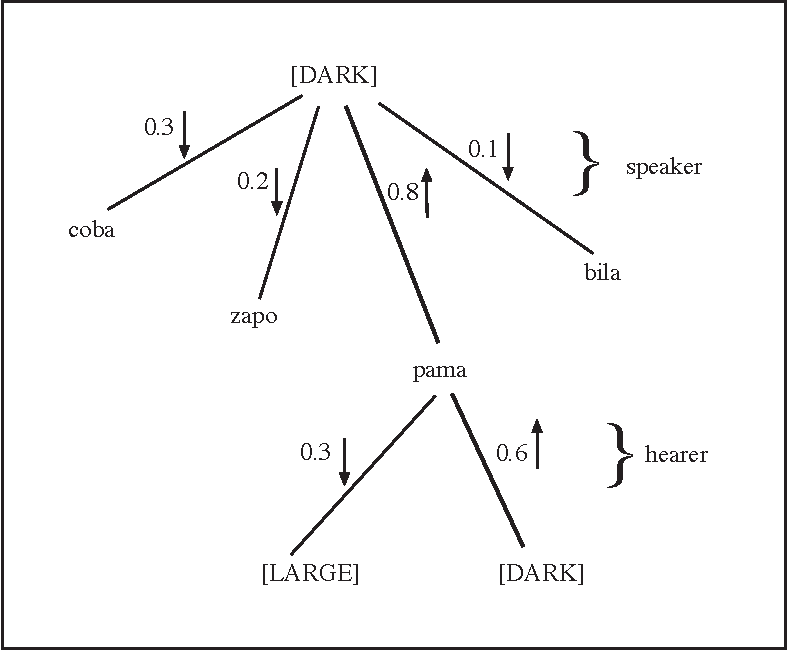
\includegraphics[width=.60\textwidth]{chap5/figs/incr-decr}}
\caption{ \label{incr-decr} 
Score adjustments after a successful game. Scores of used 
associations go up and their competitors go down.}
\end{figure}

It is possible to impose an even stronger\is{lateral inhibition}
lateral inhibition, by assuming that in the case of 
success, the speaker decreases the score of 
all the associations that imply the word used in 
the game but with another meaning, and the 
hearer decreases the score of all the associations
that imply the same meaning but with another 
word. This obviously requires additional processing
from the side of the agents. 

\subsection{Constructing and acquiring words}

When virgin agents start playing naming games, their 
associative memories are completely empty. Each agent 
needs two additional activities to get a lexicon
emerging: 
\begin{itemize}
\item 
When an agent does not have a word for a
meaning he wants to communicate, he is allowed to create
a new word (by random combination of vowels and 
consonants) and add that to his 
lexicon. Agents are assumed to have a 
shared repertoire of syllables which they can all 
produce and recognise. This happens with a certain 
probability, the {\it word creation rate} $w_{c}$. 
This rate reflects how `free' the agent feels to 
extend the lexicon. 
\item 
When an agent hears a word he has 
never heard before, he may add this new word to his 
repertoire. Again this happens with a certain
probability, the {\it word absorption rate} $w_{a}$. 
This rate reflects the critical attitude with which an 
agent accepts the linguistic authority of other agents. 
\end{itemize}
These rates are not critical but must of course
be positive. Experiments continue to work 
when agents always make a new word ($w_{c}=1$) 
and always absorb the word of the other ($w_{a}=1$). 

\subsection{The Naming Game in action}
 
To become more familiar with the Naming Game, I will now 
go through a few examples of its application, assuming 
a group of five agents: ${\cal A}$ = $\{${\bf a1},{\bf a2},
{\bf a3}, {\bf a4}, {\bf a5}$\}$ and five possible shared meanings: 
\newline 
${\cal M}$ = $\{[DARK],[LARGE],[LIGHT],[SMALL],[RED]\}$. 
\newline
Here is a trace of a first game as reported by 
the commentator, when the agents do not have any lexicon at
all. 
\begin{verbatim}
Game 0 
  a5 is the speaker. a3 is the hearer. 
  a5 categorizes the topic as [LIGHT]
  a5 does not have a word for [LIGHT]
\end{verbatim}
This trace lists the number of the game, the speaker, the 
hearer and the categorization of
the topic. The speaker did not have a word and did not 
create one (because the word creation probability is 
$w_{c}=0.1$): the game has failed. In the beginning 
most games fail if the word creation rate has been set to a low rate.

In the next game shown below, the speaker is 
{\bf a4}, the hearer {\bf a5} and the topic
[SMALL]. Now the speaker is successful in creating a word, namely 
"di". The hearer receives the word, does not know it,
but stores it in association with [SMALL]. The game still fails. 
\begin{verbatim}
Game 29
   a4 is the speaker. a5 is the hearer. 
   a4 categorizes the topic as [SMALL]
   a4 creates a new word: "di"
   a5 does not know "di"
   a4 points to the topic
   a5 categorizes the topic as [SMALL]
   a5 stores "di" as [SMALL]
\end{verbatim}
In game 32, something similar happens. This time {\bf a5} creates
a new word "pida" for [LARGE]. {\bf a3} does not know 
the word but stores it. 
\begin{verbatim}
Game 32
   a5 is the speaker. a3 is the hearer. 
   a5 categorizes the topic as [LARGE]
   a5 creates a new word: "pida"
   a5 says: "pida"
   a3 does not know "pida"
   a5 points to the topic
   a3 categorizes the topic as [LARGE]
   a3 stores "pida" as [LARGE]
\end{verbatim}
A first success occurs in game 43, when {\bf a5} uses again 
"pida" for [LARGE]. {\bf a3} hears "pida", has associated it 
in his lexicon with [LARGE], and so the game succeeds. 
\begin{verbatim}
Game 43
   a5 is the speaker. a3 is the hearer. 
   a5 categorizes the topic as [LARGE]
   a5 says: "pida"
   a3 interprets "pida" as [LARGE]
   a3 points to the topic 
   a5 signals OK
\end{verbatim}
It is quite tedious to go through such games by hand. 
For large populations of agents or meanings, even the 
most diligent researcher soon loses patience. Fortunately 
it is not so difficult to implement the Naming Game model on 
a computer. This makes large-scale simulations, even with 
hundreds of agents and meanings feasable, and ensures
that they have been done correctly.
All traces and graphs of games reported in this book
have been produced by computer simulations or physical 
experiments with the Talking Heads. 

\subsection{Characterising the Lexicon}

The individual lexicon of one
agent, {\bf a5}, after 100 games is shown in \ref{tab:t-mem3}. 
\begin{table}
\begin{center}
\begin{tabular}{l  l  l }
\lsptoprule 
{\it Meaning} & {\it Word} & {\it Score} \\ \midrule
[LARGE]& pida& 0.20\\ \midrule
  & fobu& 0.1\\ \midrule
[LIGHT]& gi& 0.0\\ \midrule
[SMALL]& di & 0.10\\ \midrule
\lspbottomrule
\end{tabular}
\caption{\label{tab:t-mem3} Associative memory of a single agent after 100 games.}
\end{center}
\end{table}
Both the words "di" and "pida" are present but with 
weak scores. There are two synonyms for 
[LARGE]: "pida" and "fobu", but "pida" is 
preferred. There is a word "gi" who is available 
for [LIGHT] but does not have a positive score,
because successive trials failed to yield a successful game. 

A table such as the one above only represents the lexicon
of a single agent. It is highly unlikely that two agents
share the same lexicon because each agent will have 
had different encounters and hence different language
experiences. A picture of the lexicon of the group from the 
viewpoint of an outside observer can be obtained by
inspecting the internal states of each agent to 
construct the {\it group lexicon}. It groups the 
dominating meaning-form associations for all possible
meanings and the frequency of each association. 
It gives a picture of "the" lexicon 
in the group. The group lexicon
for the complete population of five agents after 50 language games
is shown in \tabref{tab:t-mem4}. 
\begin{table}
\begin{center}
\begin{tabular}{l  l  l }
\lsptoprule 
{\it Meaning}& {\it Word} & {\it Frequency} \\ \midrule 
[LARGE]& pida& 0.40\\ \midrule
[LIGHT]& gi & 0.60\\ \midrule
[SMALL]& di & 0.40\\ \midrule
\lspbottomrule
\end{tabular}
\caption{\label{tab:t-mem4} Population lexicon after 50 games}
\end{center}
\end{table}
This reflects a situation where 40 \%
of the agents prefers to name [LARGE] with
"pida". 60 \% of the agents
use "gi" for [LIGHT], and 40 \% "di" for [SMALL]. 
The other meanings ([DARK] and [RED]) do not have names yet. 

Note that the group lexicon is not known by the agents
and is not stored anywhere in the 
total system. The only information which is locally stored in each 
agent is his own lexicon, which might be quite different from that 
of the group lexicon. For example, the lexicon of {\bf a5} shown earlier
is different from the group lexicon.
{\bf a5}'s score for "gi" is 0.0
even though the word is already preferred by 60 \% of 
the agents according to the group lexicon. 
The group lexicon is a macroscopic structure that we
as observers construct from inspecting the internal 
states of the agents. 

Let us now continue the simulation. Here are two additional
games showing how "ga" propagates from {\bf a4} to {\bf a2} in 
game 101 and from {\bf a2} to {\bf a1} in game 104. 
\begin{verbatim}
Game 104
   a4 is the speaker. a2 is the hearer. 
   a4 categorizes the topic as [RED]
   a4 says: "ga"
   a2 does not know "ga"
   a4 points to the topic
   a2 categorizes the topic as [RED]
   a2 stores "ga" as [RED]
\end{verbatim}
\begin{verbatim}
Game 104
   a2 is the speaker. a1 is the hearer. 
   a2 categorizes the topic as [RED]
   a1 says: "ga"
   a1 does not know "ga"
   a2 points to the topic
   a1 categorizes the topic as [RED]
   a1 stores "ga" as [RED]
\end{verbatim}
After a total of 250 games, the consensus is complete. 
The group lexicon is shown in \tabref{tab:t-mem5}. 
\begin{table}
\begin{center}
\begin{tabular}{l  l  c  l  l  c } \midrule 
{\it meaning} & {\it form} & {\it frequency} & {\it meaning} & {\it form} & {\it frequency}\\ \midrule 
[DARK]& go & 1.00 & [LARGE]& pida & 1.00 \\ \midrule 
[LIGHT]& gi & 1.00 & [SMALL]& di & 1.00 \\ \midrule 
[RED]& ga & 1.00 & - & - & -  \\ \midrule 
\lspbottomrule
\end{tabular}
\caption{\label{tab:t-mem5} Consensus in group lexicon, reached after 250 games.}
\end{center}
\end{table}
Once the agents have reached this stage, the lexicon does not 
change anymore, because all agents now prefer the same word for 
each possible meaning and would never choose another one
nor encounter another one. 

The lexicons of individual agents contain quite a few form-meaning
pairs that did not make it in the shared lexicon that gradually 
emerged. It is entirely feasable to envision a pruning mechanism 
that would eliminate from memory those form-meaning pairs whose 
success has been non-existent (for example because an agent created
it as speaker but it was never picked up by anybody else), 
or whose score has become zero (because another word became
dominant). The impact of such a forgetting
function has not been explored yet in our experiments. 

\subsection{Monitoring Average Success} 

I use various measures both for actual lexicon use and for 
the coherence and evolution of the lexicons of
the individuals to see better what is happening. 
The first and easiest measure is the {\it average game success}, 
also called the {\it communicative success}, \is{communicative success}
of a population of agents ${\cal A}$ in a set of $n$ language games. 
When this measure is graphed continuously for consecutive sets of 
games, the progress in the population
towards successful communication can be followed easily. This
is shown in \figref{success} which plots data from the 
games discussed in the previous paragraphs. We see at once that
average success climbs from a starting point of zero
to a maximum of 1.0. This can only be because a shared lexicon 
emerged in the population. 
\begin{figure}[htbp]
  \centerline{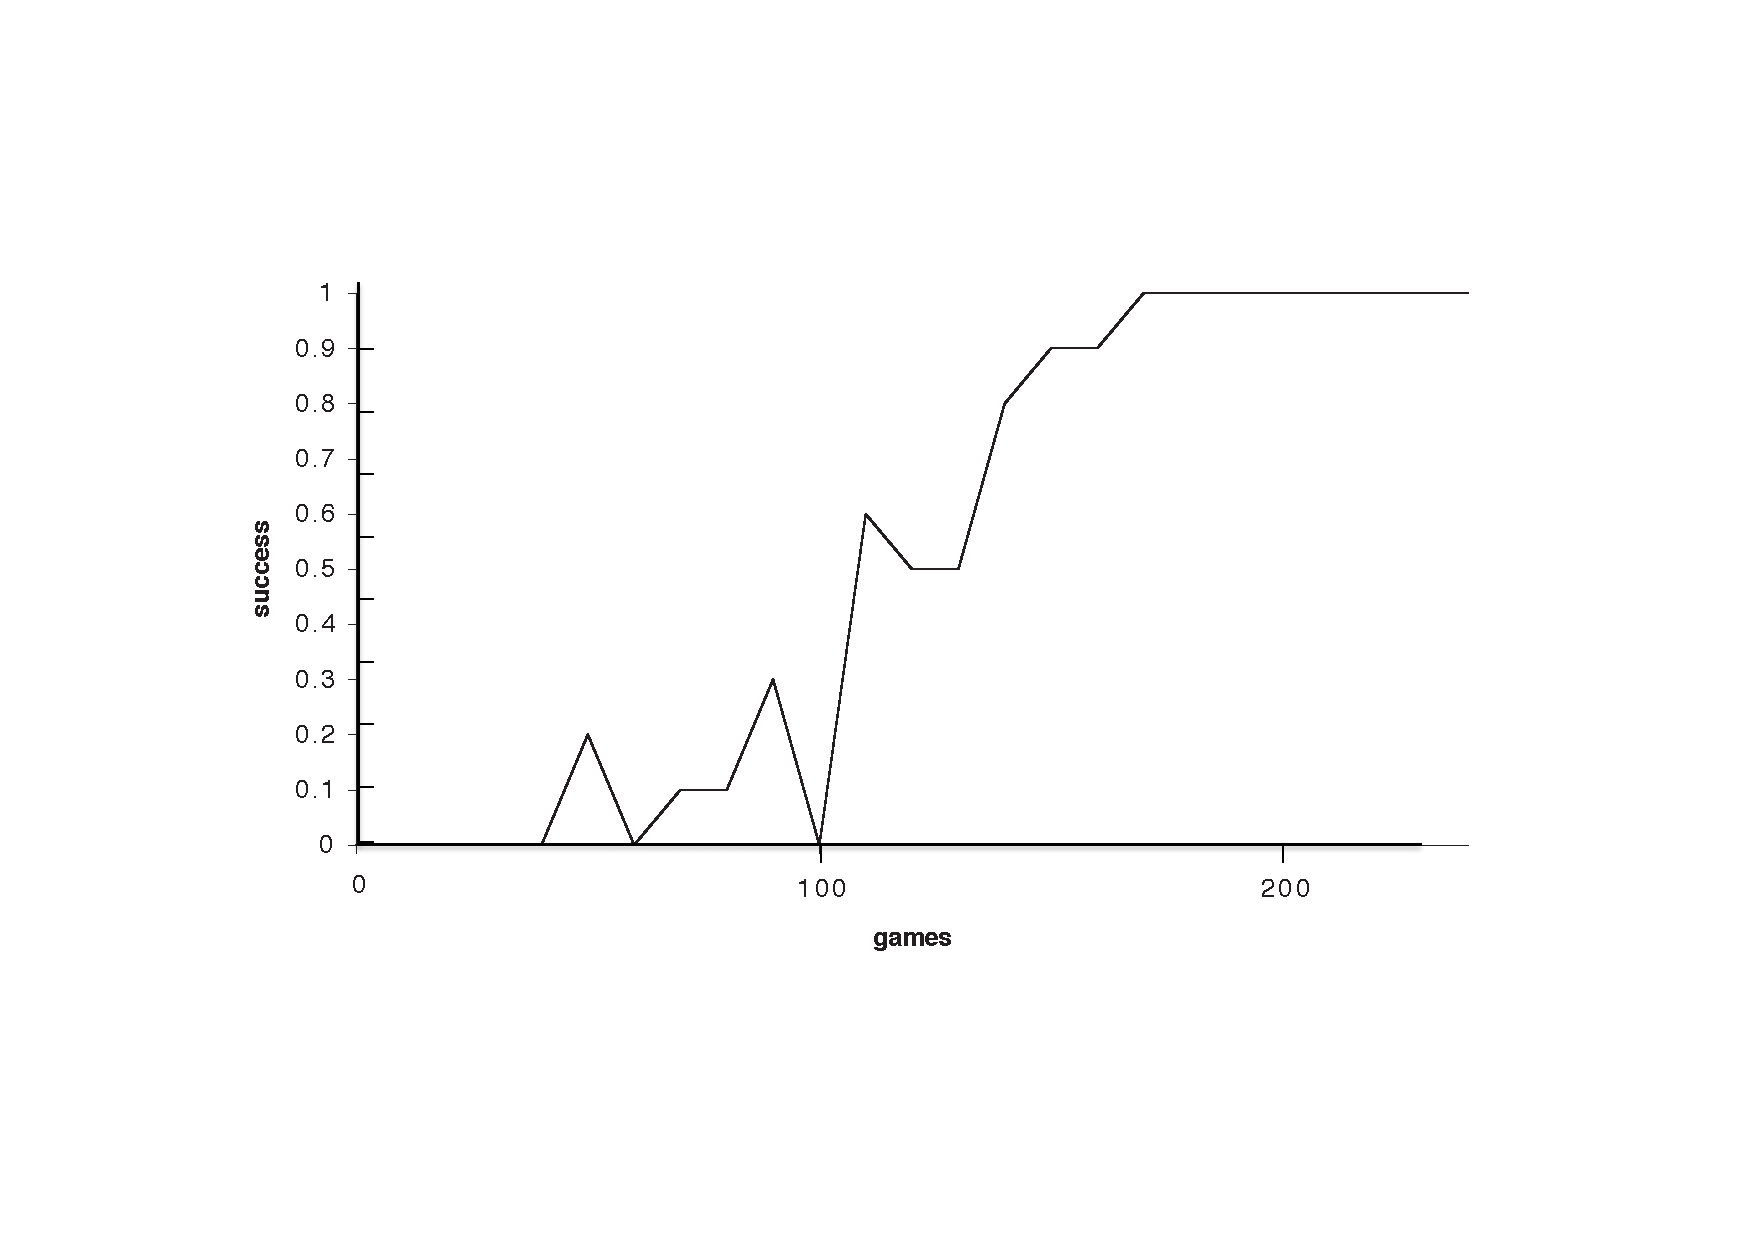
\includegraphics[width=.70\textwidth]{chap5/figs/success}}
\caption{ \label{success} 
The graph displays on the y-axis the average success every 10 games
in a population of five agents lexicalising five
different meanings. The x-axis 
shows the number of games. Average success
rapidly climbs until it reaches total success after 
about 180 games.}
\end{figure}

When the population (both of meanings and agents) is larger, 
one would expect that it takes longer to reach total average
success. This is indeed the case (\figref{larger}). 
\begin{figure}[htbp]
  \centerline{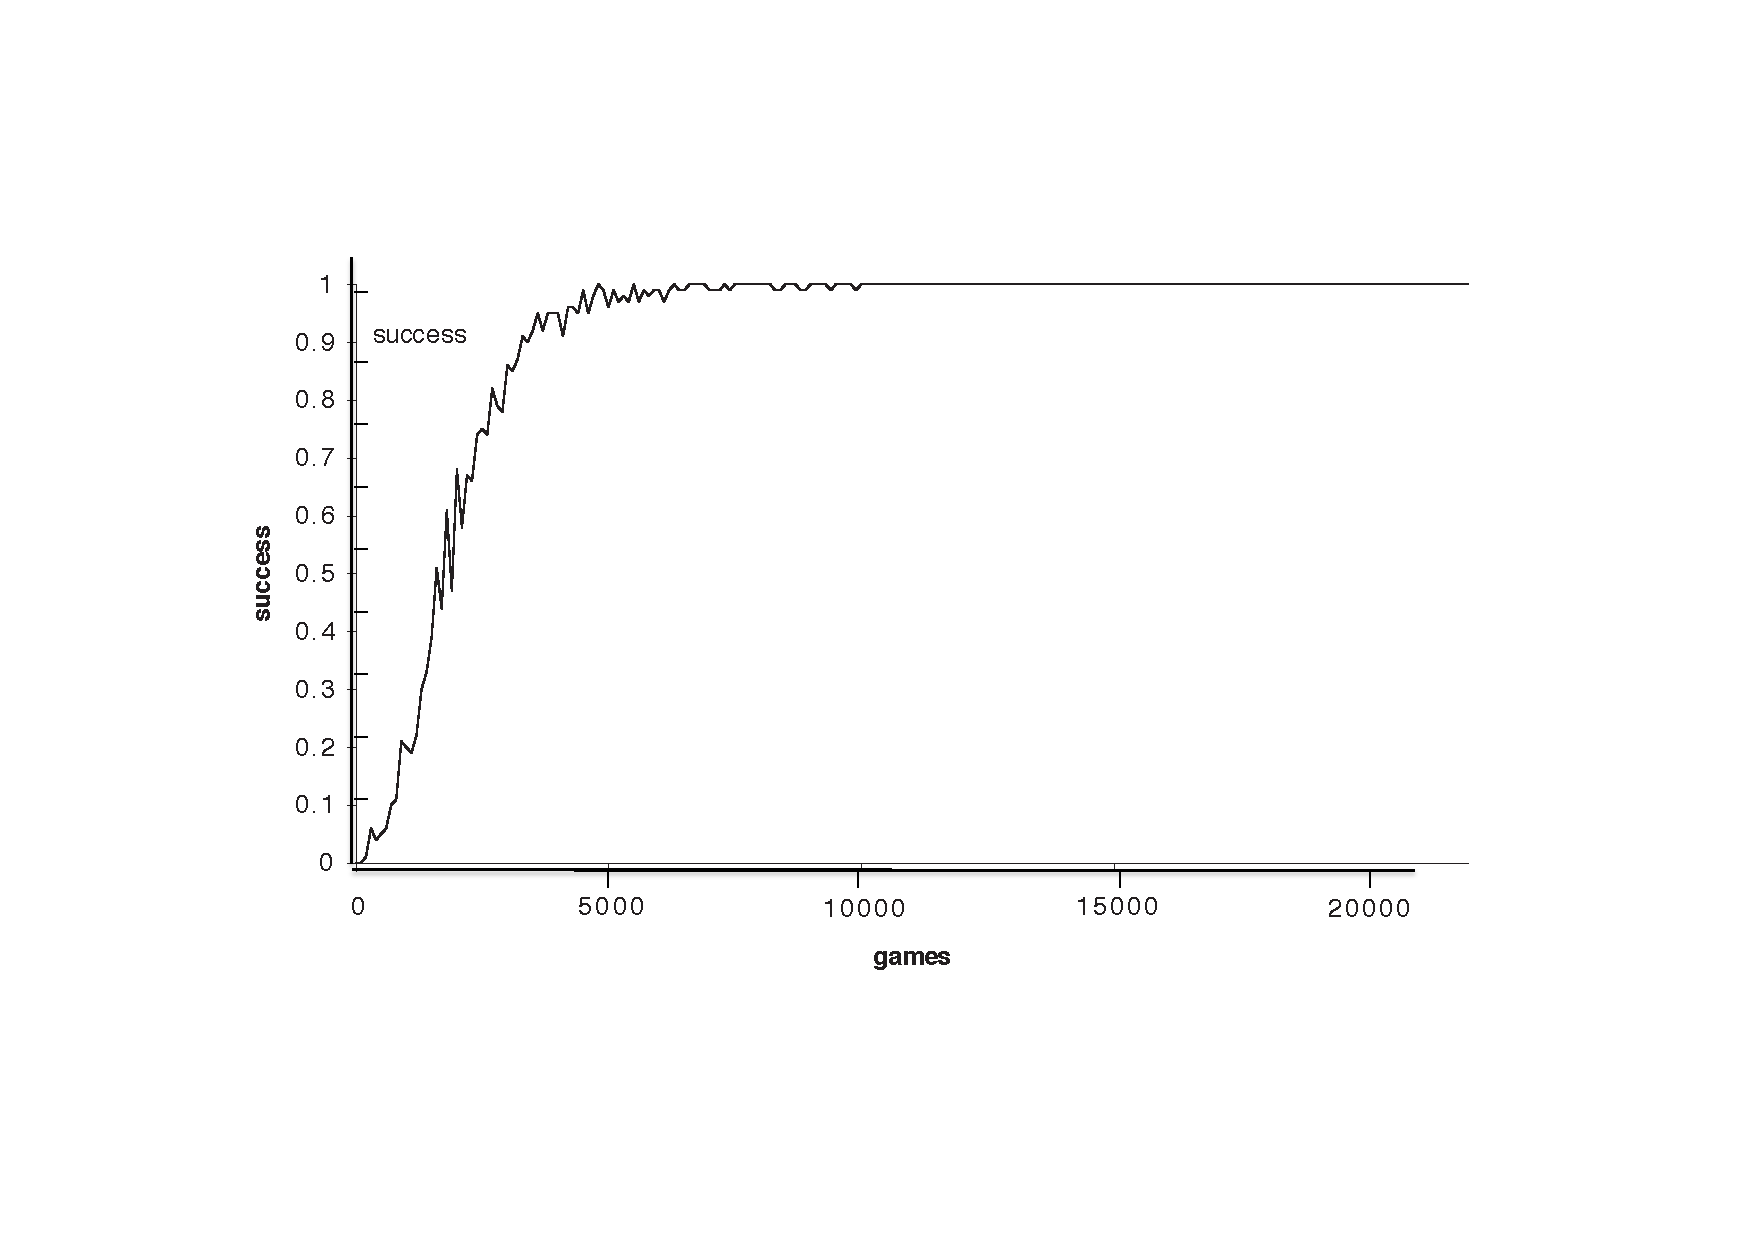
\includegraphics[width=.70\textwidth]{chap5/figs/larger}}
\caption{\footnotesize \label{larger} 
The graph displays the evolution of communicative success
for larger and larger populations. The
number of games on the x-axis
is divided by the number of agents. }
\end{figure}
We see for example that for 20 agents and 20 meanings 
success climbs to total success after about 10,000 games.
This is still surprisingly low particularly as
success is
are already above 95 \% after about 5000 games. Games can be played
in parallel by different agents because the system 
is entirely distributed. If we divide
the number of agents by the number of games, we see that about 250
games are needed by the agents to get 95 \% success, which means
that every meaning needs to appear about 10 times for each agent. 
Interestingly enough, the larger the population of agents, 
the more the success curve approximates an 
S-shape, which has 
been observed empirically in the spreading of new
linguistic conventions. The same curve shape is familiar to
biologists studying models of competitive growth, suggesting 
a strong relationships between ecological dynamics and language\is{S-shape curve}
spreading.\footnote{The S-shaped curve is discussed in \cite{McMahon:1994} p. 52. For examples
of biological models with similar properties, see \cite{May:1976}.}

\subsection{Measuring lexical coherence} 

To monitor to what extent the agents share the same
lexicon, I propose a second measure, the {\it lexical
coherence}. The lexical coherence is 
defined as the average of the frequencies of
all the form-meaning pairs in the group lexicon.
If all agents prefer the same form-meaning 
pair for all meanings, lexical coherence is 1.0. If they agree
on none, it is 0.0.\is{lexical coherence}

Consider the following group lexicon after 3000 games for the
previous simulation (with 20 agents), shown in \tabref{tab:t-mem3000}. 
\begin{table}
\begin{center}
\begin{tabular}{l  l  l  l  l  l }
\lsptoprule 
{\it meaning} & {\it form} & {\it frequency} & {\it meaning} & {\it form} & {\it frequency} \\ \midrule
[DARK]& dato & 1.00 & [LARGE]& biti & 0.80 \\ \midrule 
[LIGHT]& pitu & 0.60 & [SMALL]& dopu & 1.00 \\ \midrule 
[RED]& gabi & 1.00 & [GREEN]& gu & 0.85 \\ \midrule 
[SQUARE]& koti & 0.50 & [RECTANGLE]& totu & 0.65 \\ \midrule 
[LEFT]& toga & 0.90 & [BLUE]& ku & 0.80 \\ \midrule 
[YELLOW]& gubo & 0.55 & [CHARMING]& ge & 1.00 \\ \midrule 
[TRIANGLE]& bu & 0.85 & [SQUARE]& ba & 0.60 \\ \midrule 
[FAST]& beke & 1.00 & [SLOW]& tu & 0.95 \\ \midrule 
[CIRCLE]& ke & 0.75 & [RIGHT]& gaba & 0.95 \\ \midrule 
[UP]& butu & 1.00 & [DOWN]& ki & 0.95 \\ \midrule 
\lspbottomrule
\end{tabular}
\caption{\label{tab:t-mem3000} Group lexicon after 3000 games.}
\end{center}
\end{table}
The lexical coherence is at this point equal to 0.835. 

Lexical coherence can be graphed alongside
average success (see \figref{suc-coh}). As expected, 
lexical coherence increases 
and we can see that as coherence increases the success
rate increases.
\begin{figure}[htbp]
  \centerline{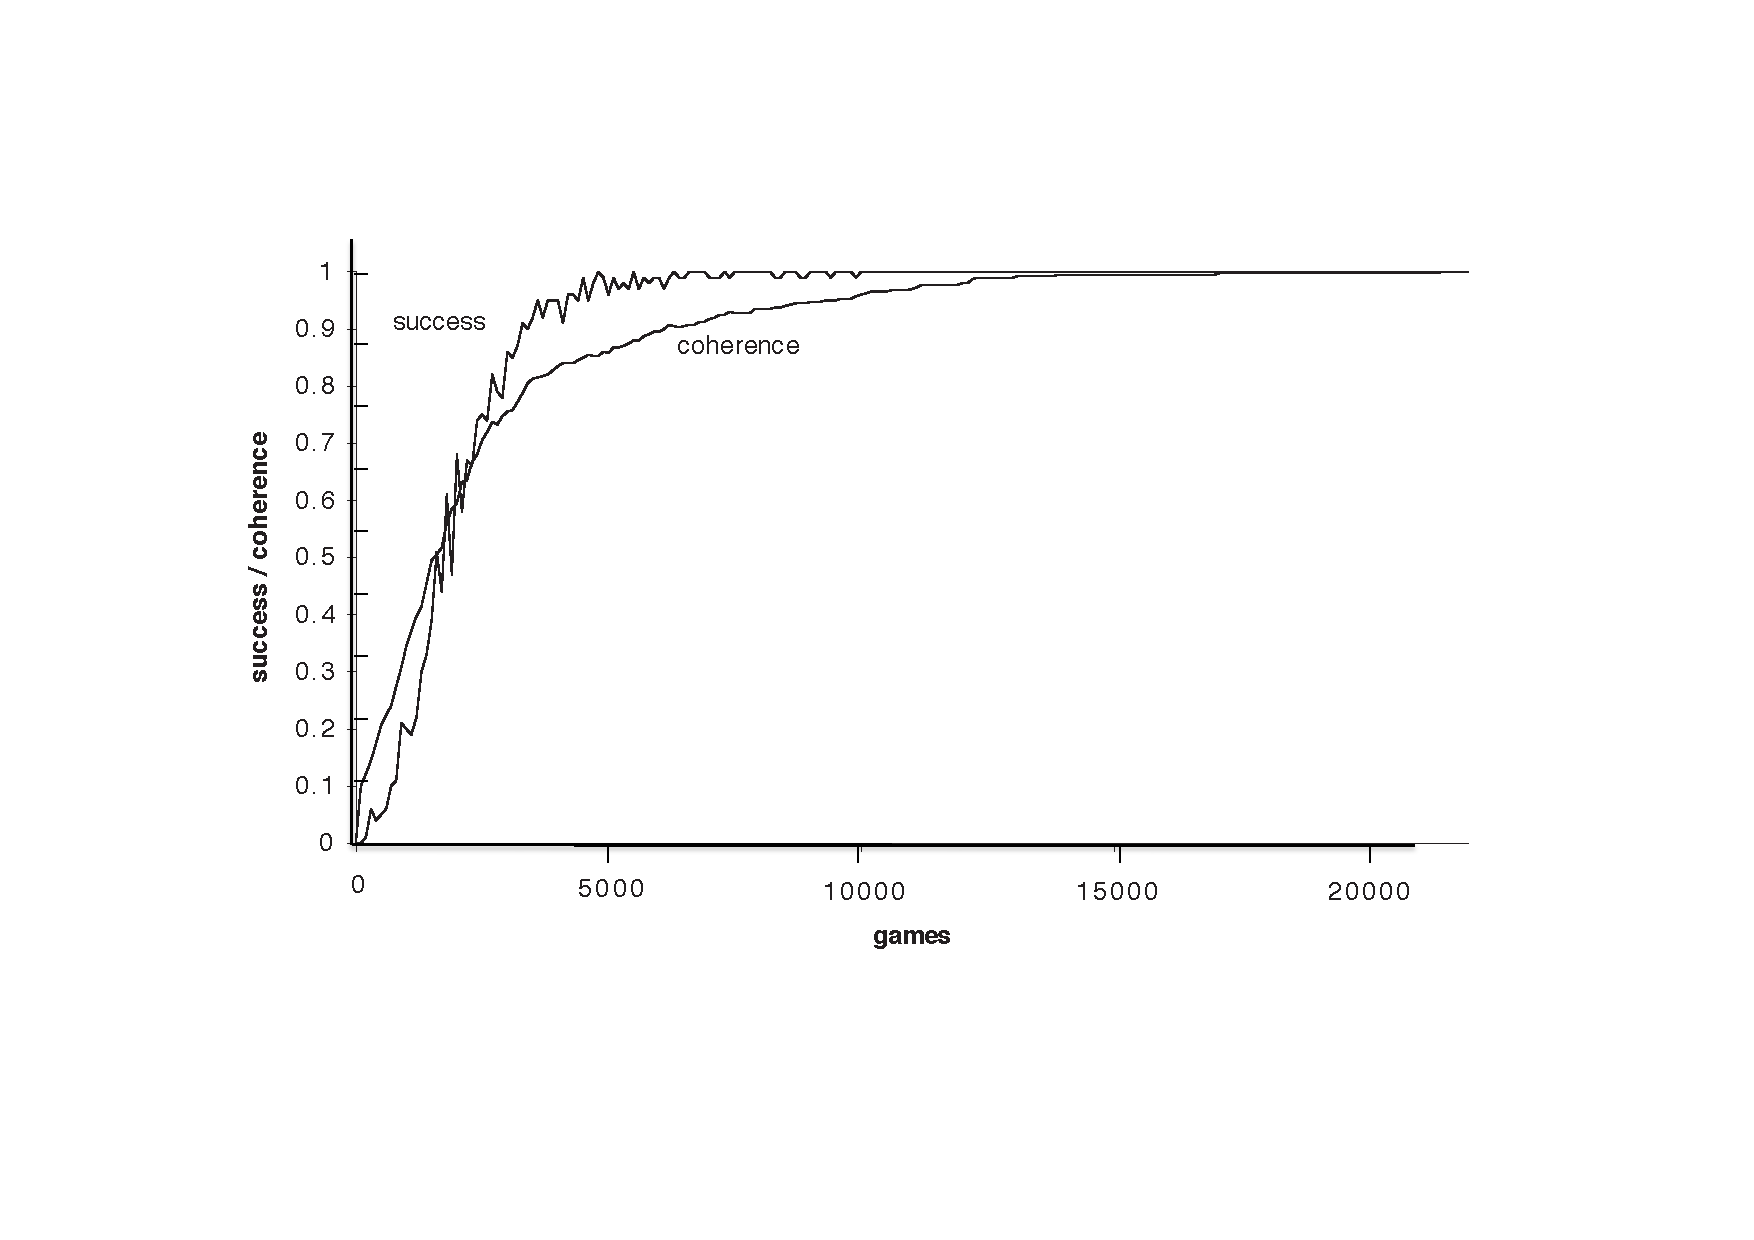
\includegraphics[width=.70\textwidth]{chap5/figs/suc-coh}}
\caption{\label{suc-coh}This figure shows the evolution of both average
success and lexical coherence for a group of 20 agents and 20 
meanings. Total lexical coherence climbs more slowly
once the 
population has reached a high average success.}
\end{figure}
Does total success imply that all agents use the 
same lexicon? Not really. To have success, the hearer
must associate the form used by the speaker
with the same meaning. But it is not required that the
hearer himself prefers to use the same form for the same meaning, 
synonyms may occur.  
A speaker of British English typically uses the word "pavement", 
whereas an American prefers "sidewalk", even though he
understands "pavement". Thus there can 
be several forms active in the same population, even though 
the outcome of a game is always successful. We will see 
later that synonyms do get damped, as is the case in 
human natural lexicons. 

Initially lexical coherence is higher than success, because a game 
fails if the hearer is acquiring the form-meaning association
used by the speaker. So two agents could have stored the same association, 
and thus coherence would have increased, without already having enjoyed the benefit
in a successful communication. However, once success
is total, agents no longer make changes based on negative feedback
from failure, simply because there is no failure,  
even the less common forms are understood correctly 
by everybody. Further progress towards more coherence
is therefore only due to the 
fact that the more common forms occur more often so that
their scores keep going up as they are used more. 

\section{Scaling up} 

The associative memory and the score updating introduced
in the previous section appears to allow a group of 
distributed agents to establish a shared repertoire of
form-meaning pairs. Of course, I still need to show that 
this mechanism remains adequate when it is incorporated
in a complete game, in which case there is no direct feedback 
about meaning. But before doing so, let us see whether 
the mechanisms are adequate from the viewpoint of scaling: 
Can they handle variation in the set of meanings to 
be expressed? Do they cope with a changing population? 

\subsection{Coping with new meanings}

In natural languages, new meanings arise every day 
while other meanings become irrelevant. 
For example, none of the terms used for talking about
the Internet (e-mail,
surfing, home page, etc.) would have made sense to anyone
a few decades ago. On the other hand, most of us now have lost 
many categories and concepts for classifying plants, 
simply because they are no longer such a prominent part of our 
urbanised environments. It follows that a mechanism 
claiming to explain the origins and acquisition 
of a lexicon in a population
of agents should cope with a fluctuating set of meanings
as well. This property is moreover crucial in the Talking 
Heads experiment because new meanings will continuously 
arise as the agents encounter new situations in 
the environment. 

Because the Naming Game included ways to 
handle new meanings from the start, nothing should 
have to be changed to handle an increased set of meanings. 
Let us see whether the Naming Game indeed copes
through the next simulation (see \figref{inoutmean}), using 
arbitrary labeled meanings ([M1], [M2], etc.). 
In a first phase, the system is closed 
and a shared lexicon emerges for the initial set 
of 20 meanings, as expected. The group's lexicon
is now as in \tabref{tab:gphase1}. 
\begin{table}
\begin{center}
\begin{tabular}{l  l  c  l  l  c } \midrule 
{\it meaning} & {\it form} & {\it frequency} & {\it meaning} & {\it form} & {\it frequency}\\ \midrule 
[M1]& gebo & 1.00 & [M2]& goge & 1.00 \\ \midrule 
[M3]& koto & 0.70 & [M4]& da & 1.00 \\ \midrule 
[M5]& peko & 1.00 & [M6]& ki & 1.00 \\ \midrule 
[M7]& gipe & 1.00 & [M8]& kedo & 1.00 \\ \midrule 
[M9]& do & 1.00 & [M10]& gige & 1.00 \\ \midrule 
[M11]& pi & 1.00 & [M12]& bu & 1.00 \\ \midrule 
[M13]& pa & 1.00 & [M14]& kipa & 1.00 \\ \midrule 
[M15]& depi & 0.95 & [M16]& pudi & 1.00 \\ \midrule 
[M17]& tegi & 1.00 & [M18]& ba & 0.90 \\ \midrule 
[M19]& ko & 1.00 & [M20]& guda & 1.00 \\ \midrule 
 \lspbottomrule
\end{tabular}
\caption{\label{tab:gphase1} Group lexicon after first phase.}
\end{center}
\end{table}
In phase 2, a relatively small meaning flux is introduced (one
new meaning every 1000 games). As can 
be seen from \figref{inoutmean}, 
the population copes with the change. New words are created and 
propagate in the population. The following group lexicon
shows that for newcomers like [M22] or [M25] a total 
consensus has emerged. Words for the latest
new meanings, [M28] and [M29], still have low frequencies. 
\begin{table}
\begin{center}
\begin{tabular}{ l  l  c  l  l  c } \midrule 
{\it meaning} & {\it form} & {\it frequency} & {\it meaning} & {\it form} & {\it frequency}\\ \midrule 
[M1]& gebo & 1.00 & [M2]& goge & 1.00 \\ \midrule 
[M3]& koto & 1.00 & [M4]& da & 1.00 \\ \midrule 
[M5]& peko & 1.00 & [M6]& ki & 1.00 \\ \midrule 
[M7]& gipe & 1.00 & [M8]& kedo & 1.00 \\ \midrule 
[M9]& do & 1.00 & [M10]& gige & 1.00 \\ \midrule 
[M11]& pi & 1.00 & [M12]& bu & 1.00 \\ \midrule 
[M13]& pa & 1.00 & [M14]& kipa & 1.00 \\ \midrule 
[M15]& depi & 1.00 & [M16]& pudi & 1.00 \\ \midrule 
[M17]& tegi & 1.00 & [M18]& ba & 1.00 \\ \midrule 
[M19]& ko & 1.00 & [M20]& guda & 1.00 \\ \midrule 
[M22]& to & 1.00 & [M23]& de & 0.85 \\ \midrule 
[M24]& tabo & 0.95 & [M25]& piku & 1.00 \\ \midrule 
[M26]& ku & 1.00 & [M27]& pugu & 1.00 \\ \midrule 
[M28]& tete & 0.35 & [M29]& todu & 0.35 \\ \midrule 
\lspbottomrule
\end{tabular}
\caption{\label{tab:phase1} Group lexicon after second phase.}
\end{center}
\end{table}
Next (phase 3 in \figref{inoutmean}) a much higher 
meaning flux is imposed (one new meaning every 100 games). 
Lexical coherence decreases and
average success plummets. There is not enough time to propagate
the new conventions in the group. 
Note that lexical coherence drops slower than 
success when the lexicon disintegrates. 
Coherence is based on the average for all 
meanings, thus only the new ones are therefore affecting overall coherence. 
Success drops more rapidly 
because of the high rate of failure of new meanings. 

\begin{figure}[htbp]
  \centerline{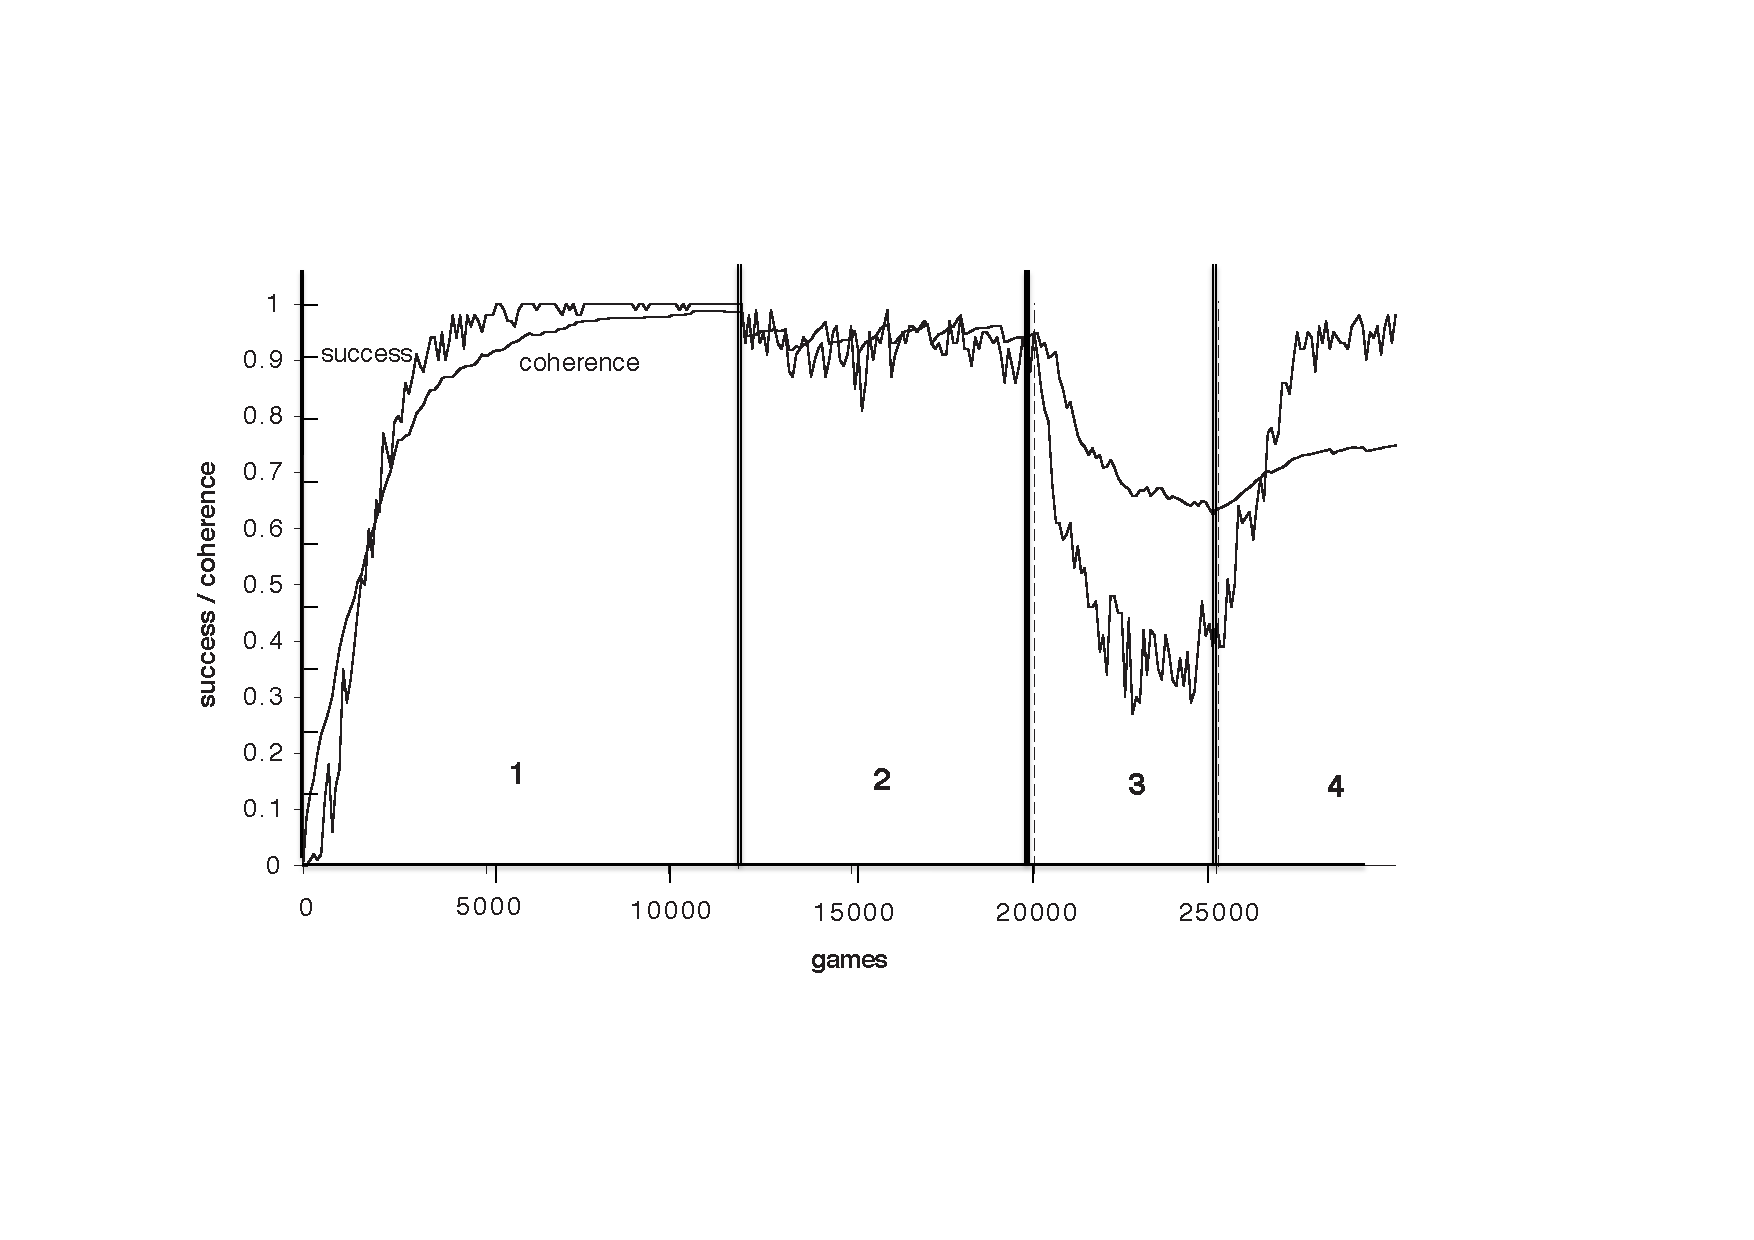
\includegraphics[width=.70\textwidth]{chap5/figs/in+out}}
\caption{ \label{inoutmean}  Both average success (every 100 games) and lexical coherence 
is shown in cases of an inflow of meanings for a population 
of 20 agents starting with 20 meanings (phase 1). The inflow 
is 1/1000 in phase 2, 1/100 in phase 3 and 1/1000 in phase 4.}
\end{figure}

The system restores itself
when the flux of meaning is brought back to 1/1000 games
(phase 4). Interestingly enough, coherence now increases slower
than success. 
The instability caused by a rapid influx of new meanings has lead 
to many new forms for the same meanings. These synonyms
now spread in the population and lead to a rapid
increase in communicative success. Coherence
climbs up more slowly because competing synonyms 
are only gradually weeded out, based on their frequency of use. 

We can conclude that the agent architecture
manages to handle an influx of meaning, as long as the flux 
stays within certain bounds. 

\subsection{Lexicon acquisition by virgin agents}

The next question we need to investigate
is whether the mechanisms 
explain how a lexicon, once it has formed, can 
be preserved from one generation to the next. This clearly 
happens in human populations. Although lexicons show
profound change, large parts get preserved even over 
very large periods of time. 
Some linguists even claim that the roots of certain 
words still in use today go back to the very beginnings
of language which is hypothesised to 
have been around 50,000 
years ago.\cite{Ruhlen:1994}
A genetic solution, where the lexicon is stored in the genetic 
code and thus transmitted from parent to child, seems clearly 
out of the question. Nevertheless, a lot of the 
early work on computational modeling
of language origins relied on a genetic approach 
for transmitting the lexicon, possibly with some
additional adaptation. See for example: \cite[603--631]{MacLennan:1991}.
This approach sheds light on the issue how signaling
systems may evolve in animals but is not applicable
to the transmission of human lexicons. The lexicon of human languages 
is too diverse and changes too quickly to allow genetic
transmission. So lexicons must somehow be transmitted 
in a cultural process.

It turns out that the agent architecture I introduced
in the previous sections does not 
need to be changed at all to obtain a cultural 
transmission of a lexicon, illustrating the explanatory 
power of the model despite its simplicity. New virgin agents
entering the group may occasionally create a new word, 
if they do not have one themselves, but if a 
particular set of words with particular meanings
is already strongly entrenched in the population, these
new words have a very low probability to survive.
Instead, the virgin agents will adopt the words
that they abundantly hear in their environment, and the
score of these words goes up quickly. 

Here is a computer simulation testing whether this 
is indeed the case (see \figref{birth}). 
We begin with a population of 20 agents and let them develop a 
shared lexicon for 20 meanings (phase 1). Then I {\it add}
new virgin agents at regular time intervals, at a rate 
of 1 every 1000 games (phase 2). A new 
agent has no knowledge of the existing lexicon and
therefore must acquire the lexicon present in the rest
of the group. \figref{birth} (phase 2) shows that the 
population indeed copes. A new member initially causes 
some failures in communication, but he quickly
picks up the lexicon of the community and success
moves back up. The lexicon does not change, it is 
stable against minor perturbations. 

\begin{figure}[htbp]
  \centerline{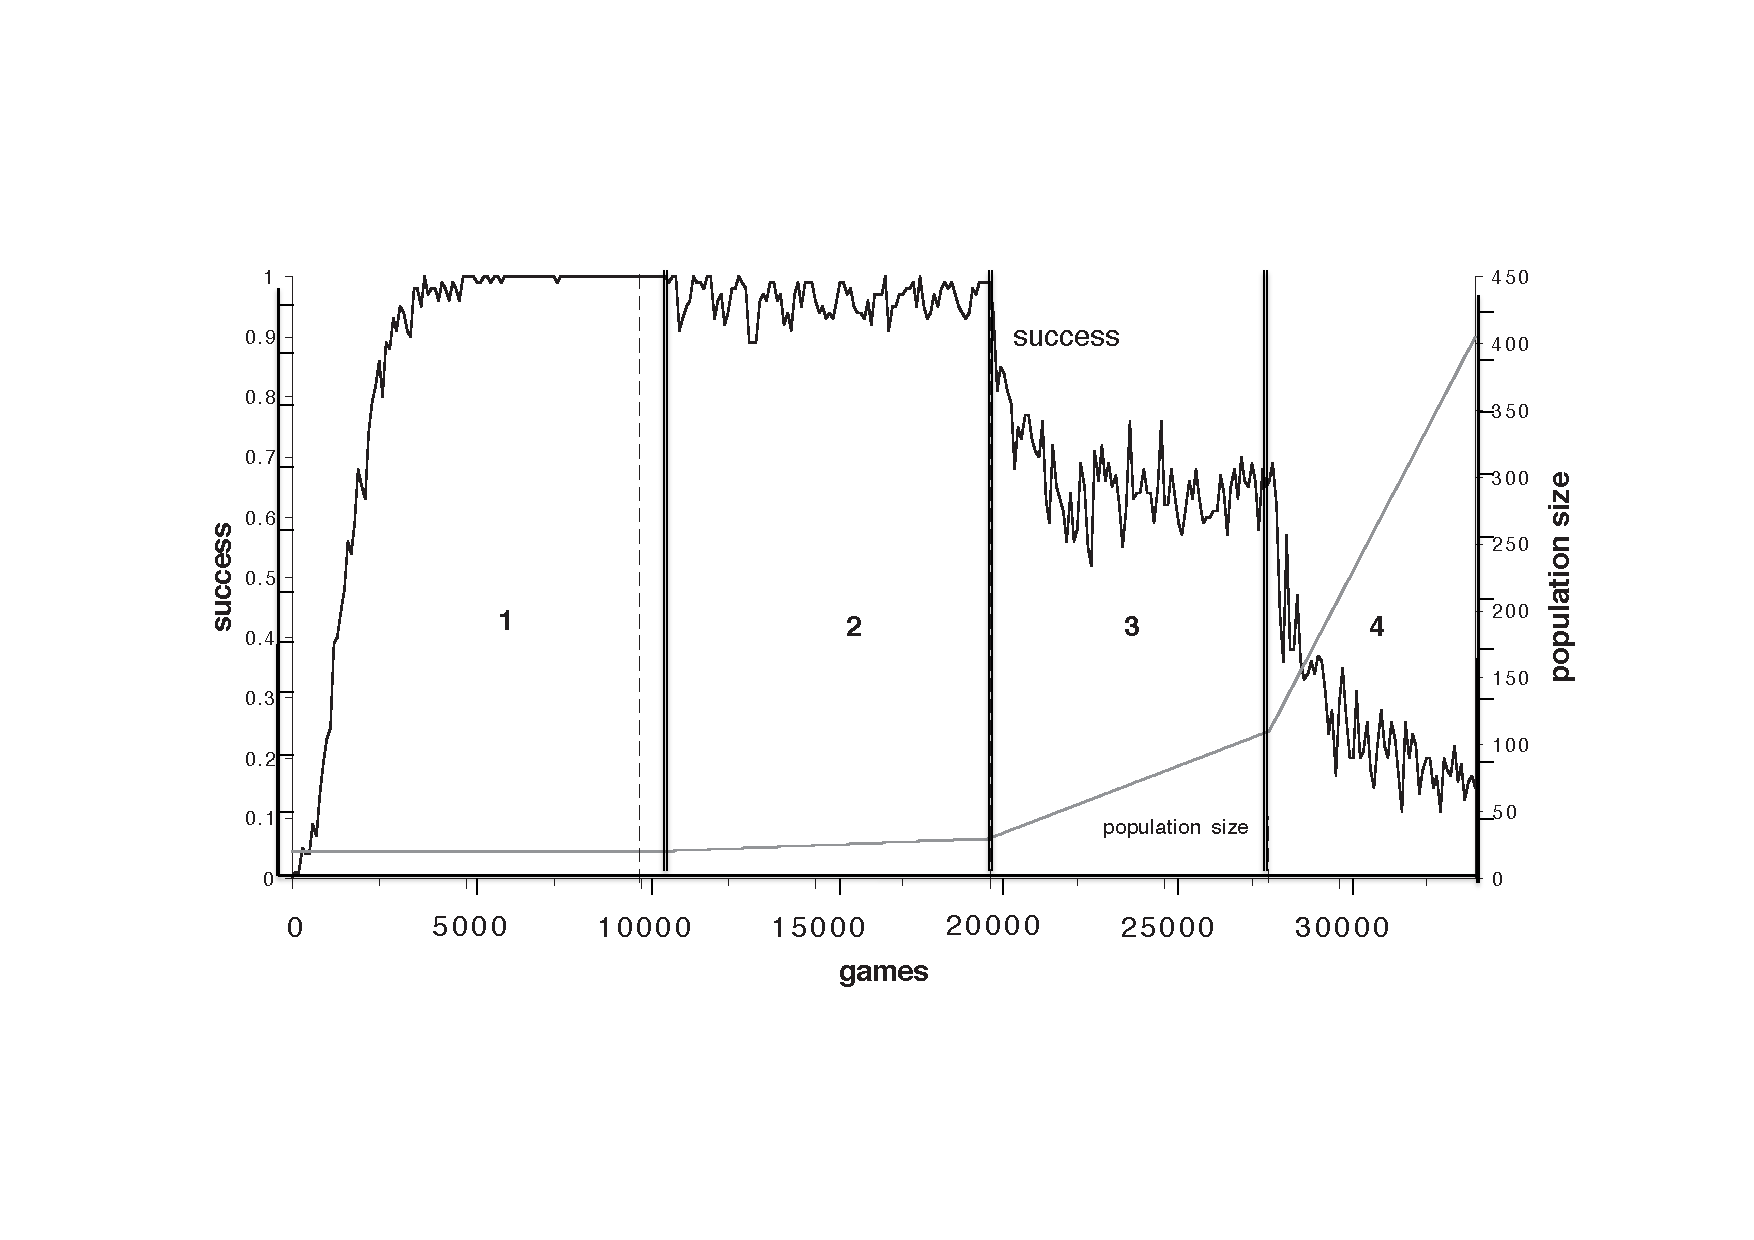
\includegraphics[width=.70\textwidth]{chap5/figs/birth}}
\caption{\label{birth} Evolution of communicative 
success with different birth-rates, starting from a
population of 20 agents (phase 1). 
Next the birth rate is increased from 1 new agent 
every 1000 games (phase 2) to 
1 new agent every 100 games (phase 3), 
and then to 1 every 50 games (phase 4).}
\end{figure}

However, when the birth rate is increased
to 1/100 games (phase 3) the population is less able to cope. 
Success stays relatively high (70 \%), but there are too many 
new agents coming in too fast. The lexicon cannot spread 
sufficiently quickly to the new agents and therefore starts 
to disintegrate. In a final stage (phase 4), the birth rate 
is set again to 1 new agent every 50 games. The population is no longer  
able to cope with the influx of new members and disintegrates. 
If inflow is brought back to a lower rate, the population would 
again establish a shared lexicon. However, 
the lexicon is now a different one
from the one that was established before. 
The dynamical process
has moved from one stable lexical state to another one.  

We have seen earlier that the Naming Game scales
up with respect to the size of possible meanings. Now 
we see that it scales up with respect to the size of 
the population. As long as the rate of influx is not too
high, the population can keep expanding. 
The only constraining factor is that new agents
must have sufficient opportunities to acquire the lexicon
present in the group. 

\subsection{Preservation in changing populations}

In human populations, there is not only an influx of 
new members but also an outflux. When somebody leaves
the community knowledge about the lexicon should
disappear as well. Nevertheless, a lexicon clearly 
gets preserved from one generation to the next, which 
implies that the know-how is distributed robustly over
the agents.\is{population change}

The next computer simulation tests whether this is also true
in the Naming Game model. 
The simulation starts with a population of 20 agents who 
are left to develop a shared lexicon for 
20 meanings (phase 1). 
Then an in- {\it and} out-flux is introduced (phase 2 in 
\figref{birth+death}) with one
new virgin agent coming in 
and another agent leaving the population every 1000 games. 
The new agent has to acquire the lexicon present in the group. 
Average success therefore dips but is quickly regained.
In fact, the population can be completely renewed without affecting the
lexicon at all. 
After 16000 games nine agents (50 \%) have been
replaced, but the lexicon has not changed. So, the Naming Game model
not only explains the formation of 
a lexicon but also its transmission: This transmission is 
entirely cultural. New agents enter the population with no 
prior knowledge. 

\begin{figure}[htbp]
  \centerline{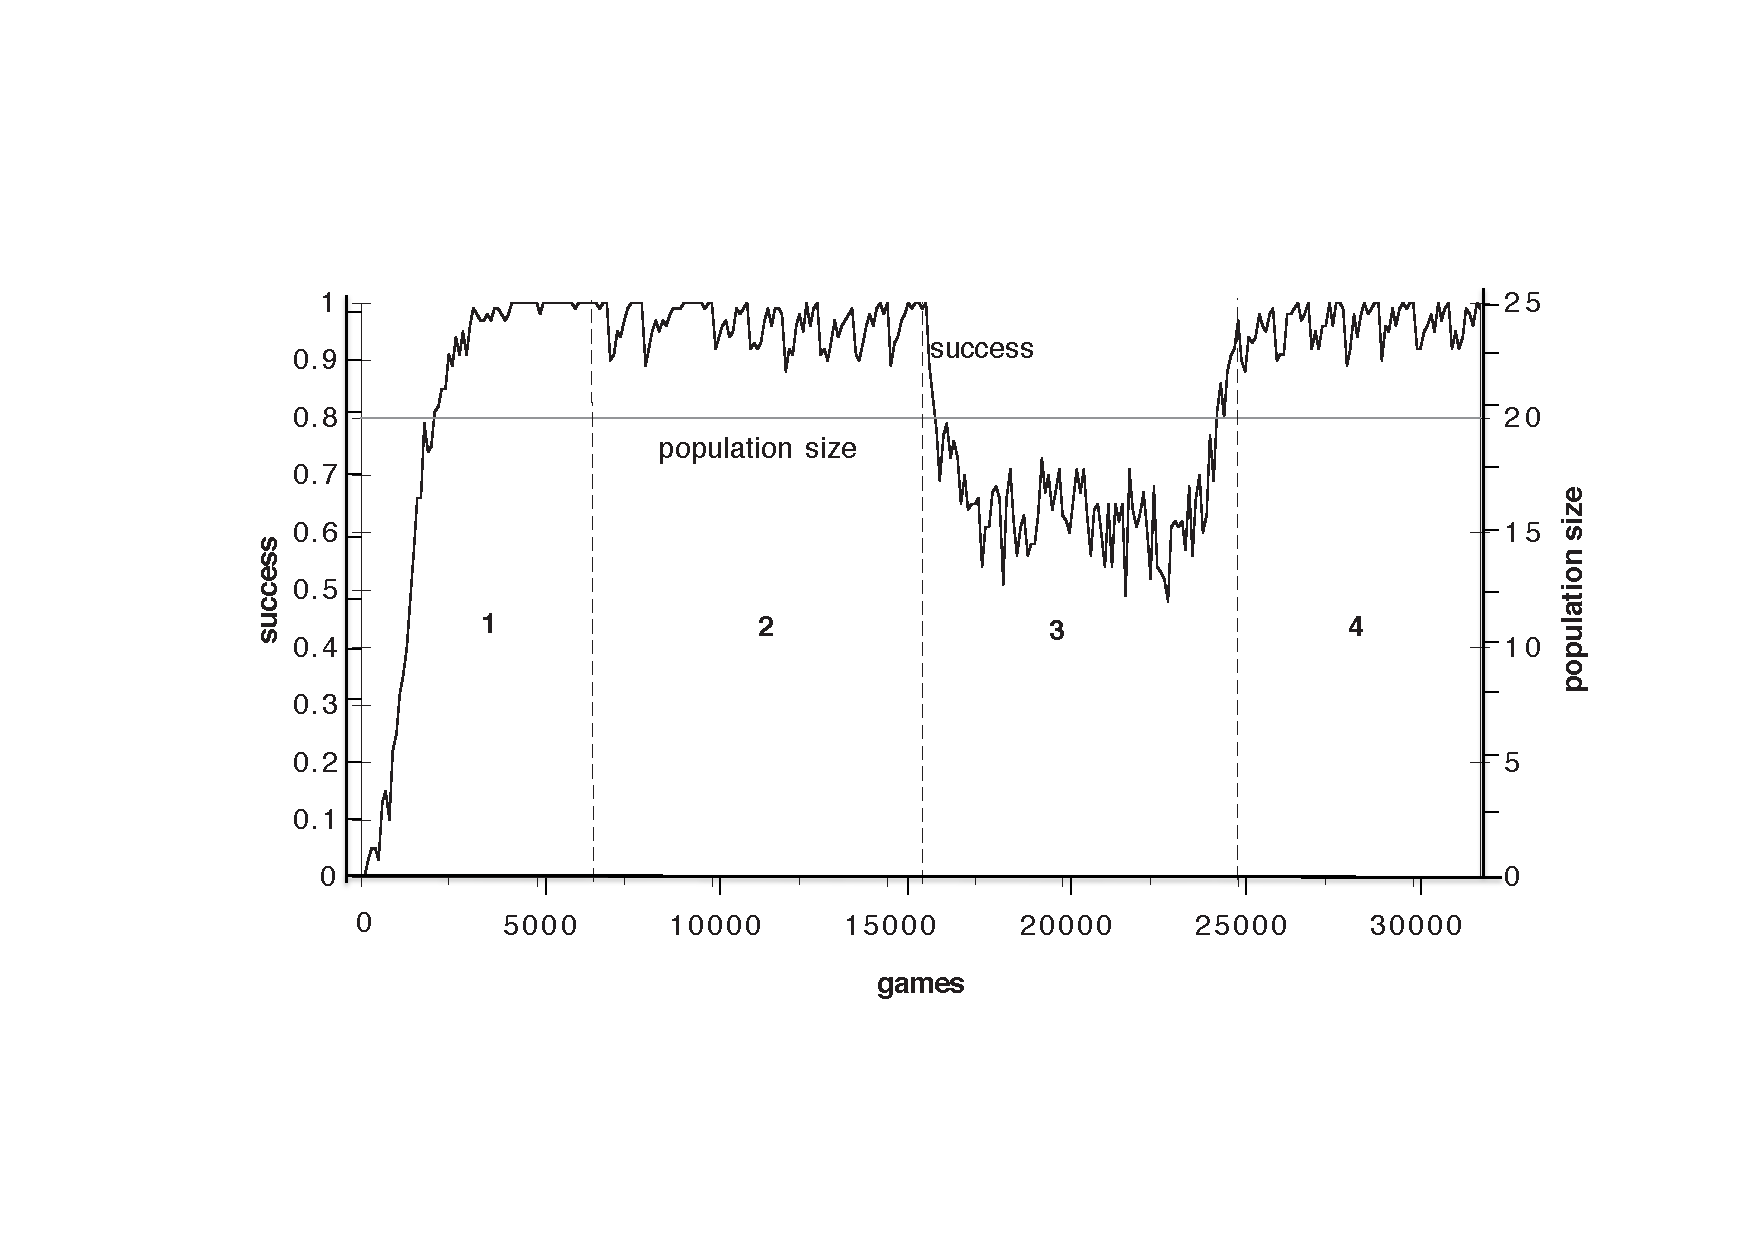
\includegraphics[width=.70\textwidth]{chap5/figs/birth+death}}
\caption{\footnotesize \label{birth+death} Success and population size 
is shown for a series of 35,000 language games. 
The population starts with 20 agents and 20 
meanings (phase 1). Then an influx and outflux is introduced 
at the rate of 1/1000 games (phase 2). The lexicon
maintains itself. In phase 3 agents enter and leave at
the rate of 1/100 games. Success lowers. In phase 
4 the rate of change is brought back to 1/1000 games
and success is regained.}
\end{figure}

Can we increase the flux in the population indefinitely? 
This is examined in phase 3 of \figref{birth+death}. 
In this phase a higher flux has been introduced. One agent is added
and removed every 100 games. Success goes down, although it is still maintained at a high 
level. The lexicon is still not changing. 
However, previous examples have already shown us 
that if we continue to increase the rate, the
lexicon would disintegrate. 
Too many new agents would be flowing in, who do not have
a lexicon yet. On the other hand, if we bring the rate of change 
back down to 1/1000 games (phase 4 in figure 
\ref{birth+death}), success regenerates. 

These simulation illustrates how we can study lexicon
transmission using a language game approach. We have
to set up an in- and outflow of the agents and 
study the impact on their communicative success
and their lexicon. In principle, we should 
not have to change the architecture of the individual 
agents, and indeed I have not done so. Language acquisition 
is such an integral part of language use that a realistic 
agent architecture must intimately integrate both capacities
from the start. Of course, at this stage 
we have only tested this
with the agents getting direct feedback about meaning, 
we still must that whether it will continue to work
with the physically instantiated Talking Heads. 

\section{Self-organisation}

These various simulations show that the Naming Game embodies robust
mechanisms for the emergence of a lexicon and we will use it 
as a core component for the Talking Heads experiment. 
In retrospect, the following mechanisms 
are crucial for the success of the model:\is{lexical self-organisation}
\begin{enumerate}
\item Agents must be able to represent multiple associations
(one form can be associated with many meanings and one
meaning with many forms). Multiple associations 
naturally arise in a population of distributed 
agents because an agent may create a new form not 
knowing that one already exists in the population, or
guess a different meaning for a form than the one
intended by the speaker. I will discuss such examples in
more detail later. 
\item An agent must be able 
to record a score for each association. The score is necessary
for the agent to decide which meaning or which form should 
be preferred in a particular interaction. When random 
choices are made lexicons do not converge. 
\item Agents must be able to create new words when no words are 
available yet. When there is a fixed set of words, the problem 
is much harder and the distributed search 
process may get stuck into local minima. 
Lexical systems must be able to cope with 
a steady influx of new meanings so restricting the set 
of words from the beginning would be odd. 
\item Agents must perform lateral inhibition, which means that 
they must decrement the score of competitors to the
form-meaning pair which won a competition. 
This is necessary to achieve convergence. 
\item Agents must get feedback in the case of failure. At the moment
the feedback is direct, but I will soon embed the naming game
into a more complex guessing game in which feedback comes
from the externally observed outcome of the language 
game as opposed to the direct transmission of the intended meaning. 
\end{enumerate}
When any of these characteristics of the agent
architecture or the game
are eliminated, the system does not work. Communicative success
does not climb, convergence will not go beyond a small percentage, 
the size of the lexicon explodes, and so on. The fact that 
these architectural properties are crucial and non-trivial to 
discover strongly suggests that similar mechanisms must be in 
place in the emergence of human lexicons. 

It is also important to stress what is not in the model. 
The mechanisms used by the agents are deliberately kept as 
simple as possible. Complexity should arise only from the 
enactment of simple construction rules. Agents do not 
go through complex reasoning about words, they simply 
store the new associations they encounter and rely on 
the updating processes to weed out wrong hypotheses. 

\subsection{Winner-take-all processes}

The most remarkable and at first mysterious property of the 
Naming Game model is that the agents somehow reach a consensus
without any central supervisor. They do {\it not} do this by 
having a general overview or by changing their internal 
parameters so as to become more conservative as the lexicon
solidifies. It is solely due to the subtle interaction between
language use, which gradually becomes uniform, and each agent's
adaptation to the language heard in the environment. 
If a certain word comes to be preferred by a group of agents
for a certain meaning, its frequency of use goes up so that
others encounter this 
word more often and hence their scores for that word
continue to increase as well.
The more agents use a word, the higher its chance of success
and the more it will be used. This effect is still enforced 
by lateral inhibition. The scores of competing associations 
decrease, making it less likely that they will win in the future. 
This positive feedback therefore introduces an\is{autocatalysis} 
{\it autocatalytic} (self-enforcing) effect until the population
locks into an equilibrium state.\footnote{
Such positive feedback loops and the stability criteria
associated with them have been widely studied in non-linear
dynamical systems and applied to chemical and biological 
processes. See \cite{Babloyantz:1986}.}

To follow better how a consensus gradually emerges, I will visualise
the competition between different words for the same meaning
in a {\it meaning-form (MF) competition diagram}, 
such as the one in \figref{competition}, which monitors 
the frequencies of the different forms in use for one meaning.
The diagram shows clearly the struggle between different forms until
one form ("pe") emerges as the winner. When we later study 
grounded lexicon formation processes, we will see that the 
competition becomes much more complex and the whole system 
is in constant evolution. A form-meaning pair which is 
dominating may become weaker because its meaning
fails to pick up the right
referent in a new context. 
This in turn may trigger the creation of new words or the 
resurgence of existing words. 
\begin{figure}[htbp]
  \centerline{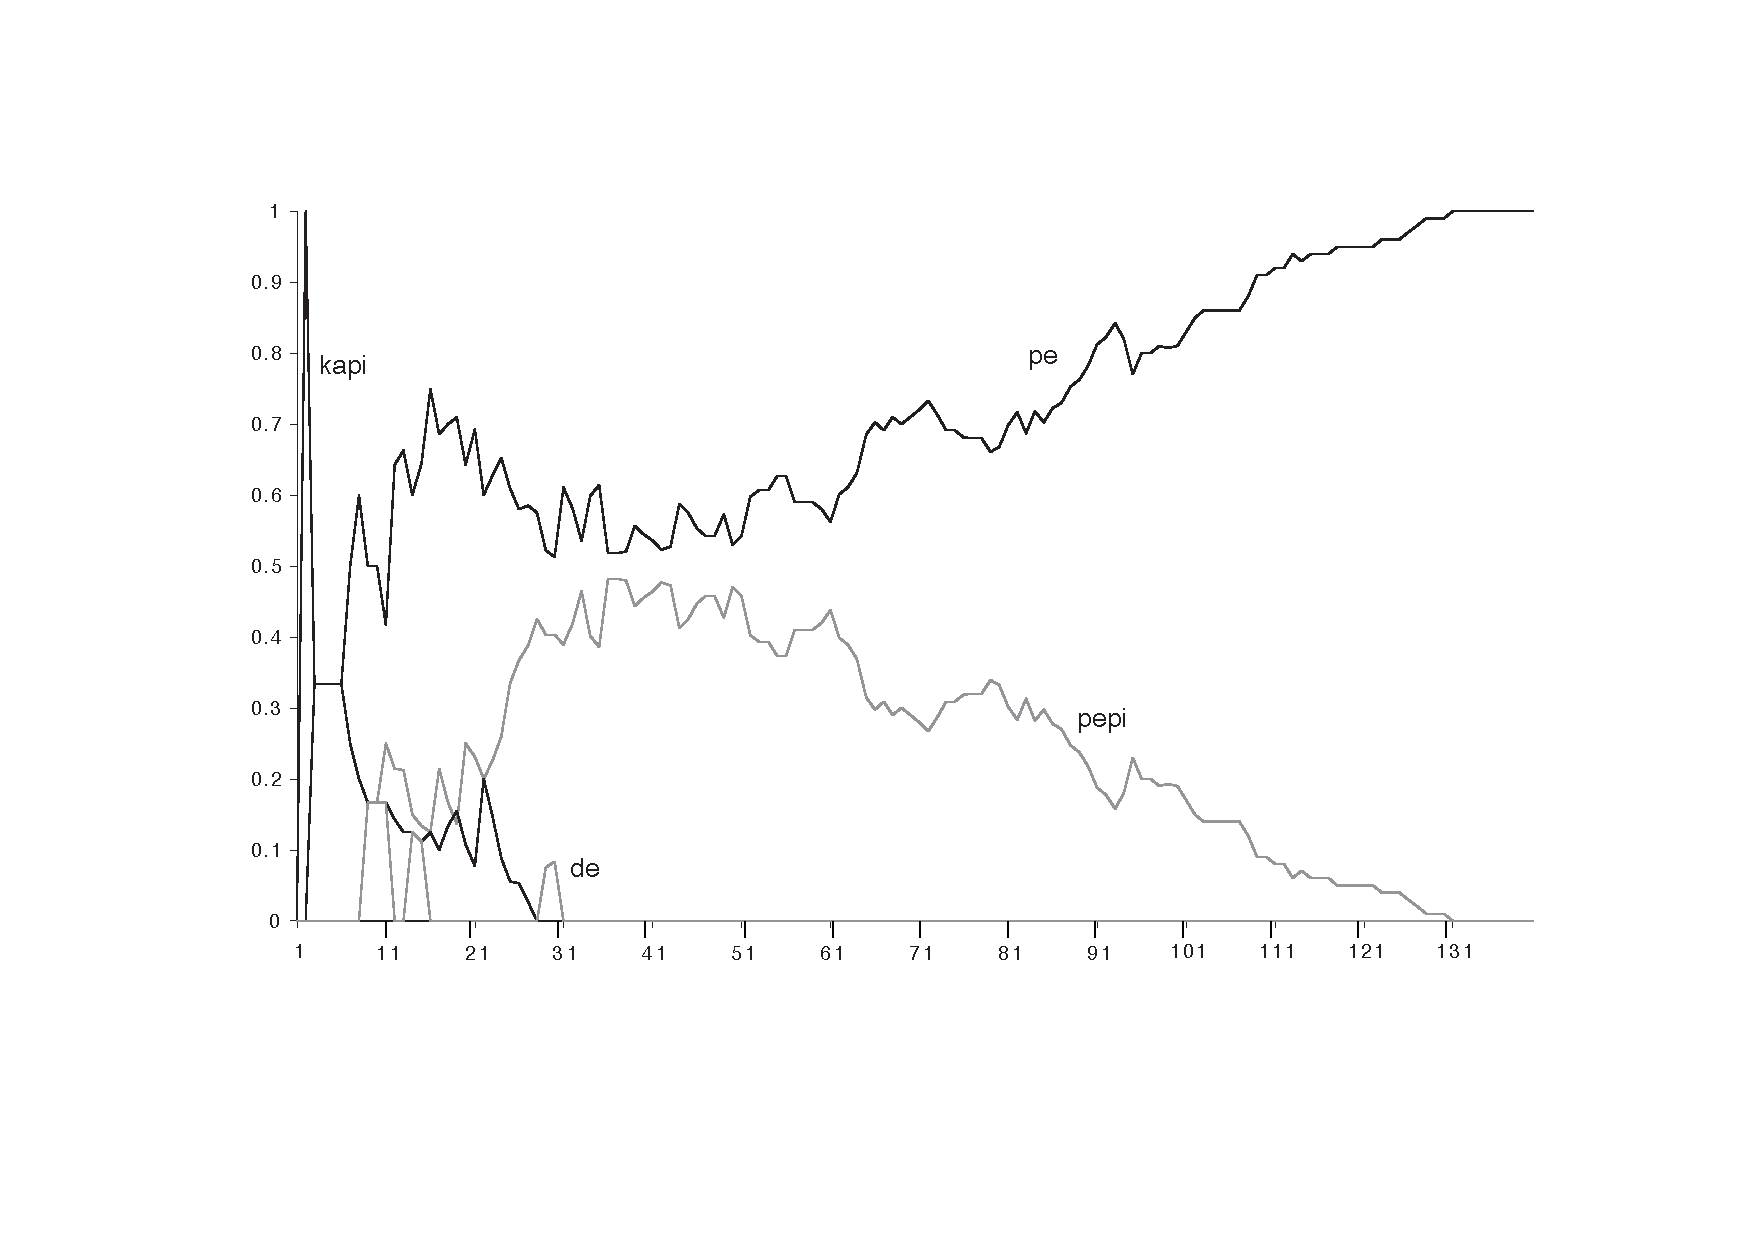
\includegraphics[width=.70\textwidth]{chap5/figs/comp1}}
\caption{\label{competition} Simulation with 
a population of 20 agents. The meaning-form competition 
diagram shows the frequency of all competing forms for a 
single meaning. We see a winner-take-all situation
with one word ("pe") dominating.}
\end{figure}

\subsection{Collective Behavior and Self-organisation}

Biology is full of examples where structures spontaneously 
self-organise from the unco-ordinated activity 
of distributed elements through a winner-take-all process.
Each time the same basic components as in the Naming Game model
are seen: Random behavior creates various possibilities and the 
reinforcement of some of these variations through positive
feedback creates an autocatalytic effect. 
Perhaps the clearest examples can be found 
in the collective behavior of 
social insects, such as the formation of nests by termites, 
although beautiful explanations have also been reported
for the formation of patterns on sea shells, the growth of
cell tissue, the aggregation
of individual cellular slime mold amoebae into a slug, 
the flocking and collective movement of birds or mammals, 
etc. (\cite{Meinhardt:1982}). A classical 
example for collective behavior, first developed by Jean-Louis 
Deneubourg, is the formation of paths in an ant society through 
mass recruitment, \cite{Pasteels:1987}. 

When ants carry food or other materials, they organise themselves in a
chain which is typically the shortest path between the source and the nest. 
These chains can sometimes be surprisingly long (20 meters is 
quite common for European ants) and are 
maintained as long as the food supply lasts. The whole process has many
intriguing properties. First of all, there is
no central planning agency that regulates which food sources 
are to be explored. The coherence and co-ordination between hundreds
or sometimes thousands of ants is established in a 
completely distributed fashion. There is no dependence 
on individual ants. Ants can 
be removed from a path or new ones can be introduced randomly without too 
much interference for the stability of the path as a whole. The paths are
robust. If objects are put in the way or if the path is destroyed, 
the ants manage to reestablish it in a relatively short time span. 
The paths are adaptive. If the food supply terminates, the path 
disintegrates and a new path will appear linking the ants to an alternative 
food source. 

We see here many of the properties found in natural languages
and integrated in the Naming Game model: 
absence of central planning, no critical dependence on a 
single element, resilience to influx or outflux of elements, and
adaptation to changing circumstances. Even more interestingly, 
the ants manage to establish these dynamic paths by a process 
which is similar to the language formation process used in the 
Naming Game, namely a positive feedback loop having an autocatalytic
effect. An individual ant appears to move around in a random fashion 
while searching for a source of 
food. When a food source is discovered, the ant returns to the nest 
using a global landmark like the sun. 
The food-carrying ant also deposits a chemical substance 
known as a pheromone as he travels back to 
the nest. This pheromone influences the 
otherwise random movement of the other ants, in that ants are 
attracted by the pheromone. Thus more ants are drawn to the path and hence
led to the food source. As these ants in turn go back
to the nest they also deposit 
pheromone. This gives the self-enforcing, autocatalytic
effect: The more ants are on the path, 
the more pheromone is deposited, and therefore the stronger 
the attraction to the other ants.
Very soon all the ants which were sufficiently close 
to the path form a chain. There is no central planning agency 
needed and the whole system does not depend on an individual ant. The 
order is emergent. 

These simple mechanisms also explain other features of the process. 
When the food source is depleted, the ants going 
back no longer deposit pheromone. And because the pheromone is 
a chemical that evaporates, it will soon have disappeared and consequently 
the ants will return to a random movement. When a path 
is interrupted because obstacles
are put in the way or because the pheromone is temporarily removed by 
an experimenter, the ants resort back to a random movement. This introduces
a random search process 
which will eventually lead to the discovery of a connection and the 
reestablishment of the path. When two ants find two food sources one closer
than the other, the society will go for the closest source. Not because they 
exchange sophisticated signals but because the trail leading to the 
closest source will be amplified faster. Adaptivity is explained in 
terms of errors in following the path. Although ants are attracted 
to the pheromone, the attraction is only partial and 
very often (how often depends on the species)
they will go astray. This sloppiness is however a source of new discoveries. 
When a lost ant hits upon a new food source
the path formed by the whole society may gradually shift
particularly if it is more abundant.

\subsection{Increasing Returns Economics}

Self-organisation is not unique to biological phenomena,\is{increasing returns economics}
on the contrary, similar situations have been intensively
studied in economics, where
the complex adaptive systems paradigm has recently also 
lead to many interesting new insights (\cite{Arthur:1996}). 
For certain types of products, particularly in 
information technology where the cost of manufacturing 
and distribution is negligable compared to the cost
of design, a winner-take-all situation can be observed. 
One product, for example a particular operating system or 
a particular microprocessor, comes to dominate the market. 

Brian Arthur and others have analysed these economic situations 
and identified a positive feedback loop as being the ultimate cause.
The more customers choose a product, the more 
others are attracted to it, particularly because 
other suppliers develop useful derivative products. Prices can 
be decreased keeping newcomers out of the market and 
customers get locked in, unable to move to other suppliers
because they have invested too much and became dependent. 
For the companies who manage to manoeuver their products
in such a situation there is a bonanza of increasing returns. 
This contrasts with the decreasing returns familiar 
from traditional equilibrium economics, where there is 
a damping of profits due to proliferating production and 
distribution cost as a product's market share increases. 

\subsection{Lessons from Nature}

The analogies between self-organisation 
in language and other fields is important for three reasons. 
First of all, if self-organisation is ubiquitous in nature
and has succesfully explained so many phenomena, its incorporation
into a model of language becomes independently motivated, and
therefore the explanatory force of the model increases. 
What is new and different is that the principle is applied
to a non-material self-organising entity, but nevertheless
the same sort of dynamics can be seen. 

Second, the large arsenal of 
mathematical tools and analysis techniques
developed in the sciences of complexity over the past decades
can be carried over to the study of language. For example, 
the mathematical models of economists like 
Arthur or biologists like Deneubourg help us develop 
mathematical explanations why language reaches coherence if autocatalysis
is present.

Third it suggests many aspects of the mechanisms
which might be relevant for language. For example, the errors ants make 
in following a trail allow them to discover occasionally 
better food sources. Could such stochasticity also play a role 
in the adaptive capabilities of language? The chaotic regime
seen in many natural systems is known to be a source
of new order.\cite{Kaneko:1996}. Could language innovation 
also be explained that way? In other words, is it possible  
that language may occasionally exhibit a chaotic
dynamics out of which new order emerges?

\section{Lexical dynamics} 

This discussion begins to illustrate a major theme 
of the present book, namely that language as a 
macroscopic phenomenon can be viewed as a complex adaptive 
system with the same characteristics as other complex
adaptive systems. 

It is well known that the dynamics of language change 
are related to the dynamics of the underlying population. Basically
we can see two phenomena. On the one hand, human populations
are not fixed for ever. New children without any knowledge
of the language are born
and other members die, taking knowledge about the 
language away with them. Populations renew at a certain rate 
which is known to have a significant impact on language. 
If the population changes quickly a language
evolves more quickly and subsystems may even destabilise. 
For example, linguists have argued that English lost its 
case system due to the Black Plague which decimated the 
population so that there was not enough opportunity for 
children to acquire the existing conventions. 

Second, human populations mix. Throughout the history of 
mankind there have been migrations or intense contact 
between geographically diverse groups. This again impacts
then the languages of the groups. 
When a given population splits into groups that have no longer 
contact, their languages start to deviate. Conversely
when there is an intense and prolonged contact between languages, 
structures from one language get adopted by the other
and vice-versa. The degree of adoption depends on which 
group is dominant. Sometimes groups adopt
another lexicon while retaining their own
syntax, and sometimes they take over the syntax
while retaining their own lexicon.\footnote{
A representative example of empirical investigations into 
language dynamics is contained in \cite{Nichols:1992}. 
See also \cite{Romaine:1988}.}

These phenomena are fascinating and interesting from the viewpoint
of language evolution, and may even explain some of the characteristics
of human languages. Linguistic systems must be 
such that they can be transmitted from one generation to the next,
otherwise they will not survive. 
In the Talking Heads experiment,
new agents may enter into the group at
any time and agents are geographically distributed. 
The local interactions 
with humans at a particular site, which is a kind of language
contact between human and artificial populations, may 
impact the evolving lexicons and ontologies. 

\subsection{Spatially Distributed Naming Games}

Language game models provide us with new fantastic tools to study\is{Spatially Distributed Naming Games}
language transmission and language contact: 
We can introduce a particular dynamics in the population
in a controlled way and then study the impact on the dynamics of the 
language itself. 
I now focus on such a model to investigate the impact of 
the migratory dynamics of a population on the dynamics 
of language. We can introduce a two-dimensional 
grid and assign every agent randomly
a position on this grid. The position assignment
can be modulated so that the agents form clusters
(\figref{figure-agent-distribution}). Such 
a population structure can be thought of as a 
geographical distribution in space but might as well 
represent a social, genetic or economical structure.
We could even envision models integrating
several of these alternate dimensions. The physical 
Talking Heads network connecting installations in 
different geographical locations allows to do these 
experiments for real. 
\begin{figure}[htbp]
  \centerline{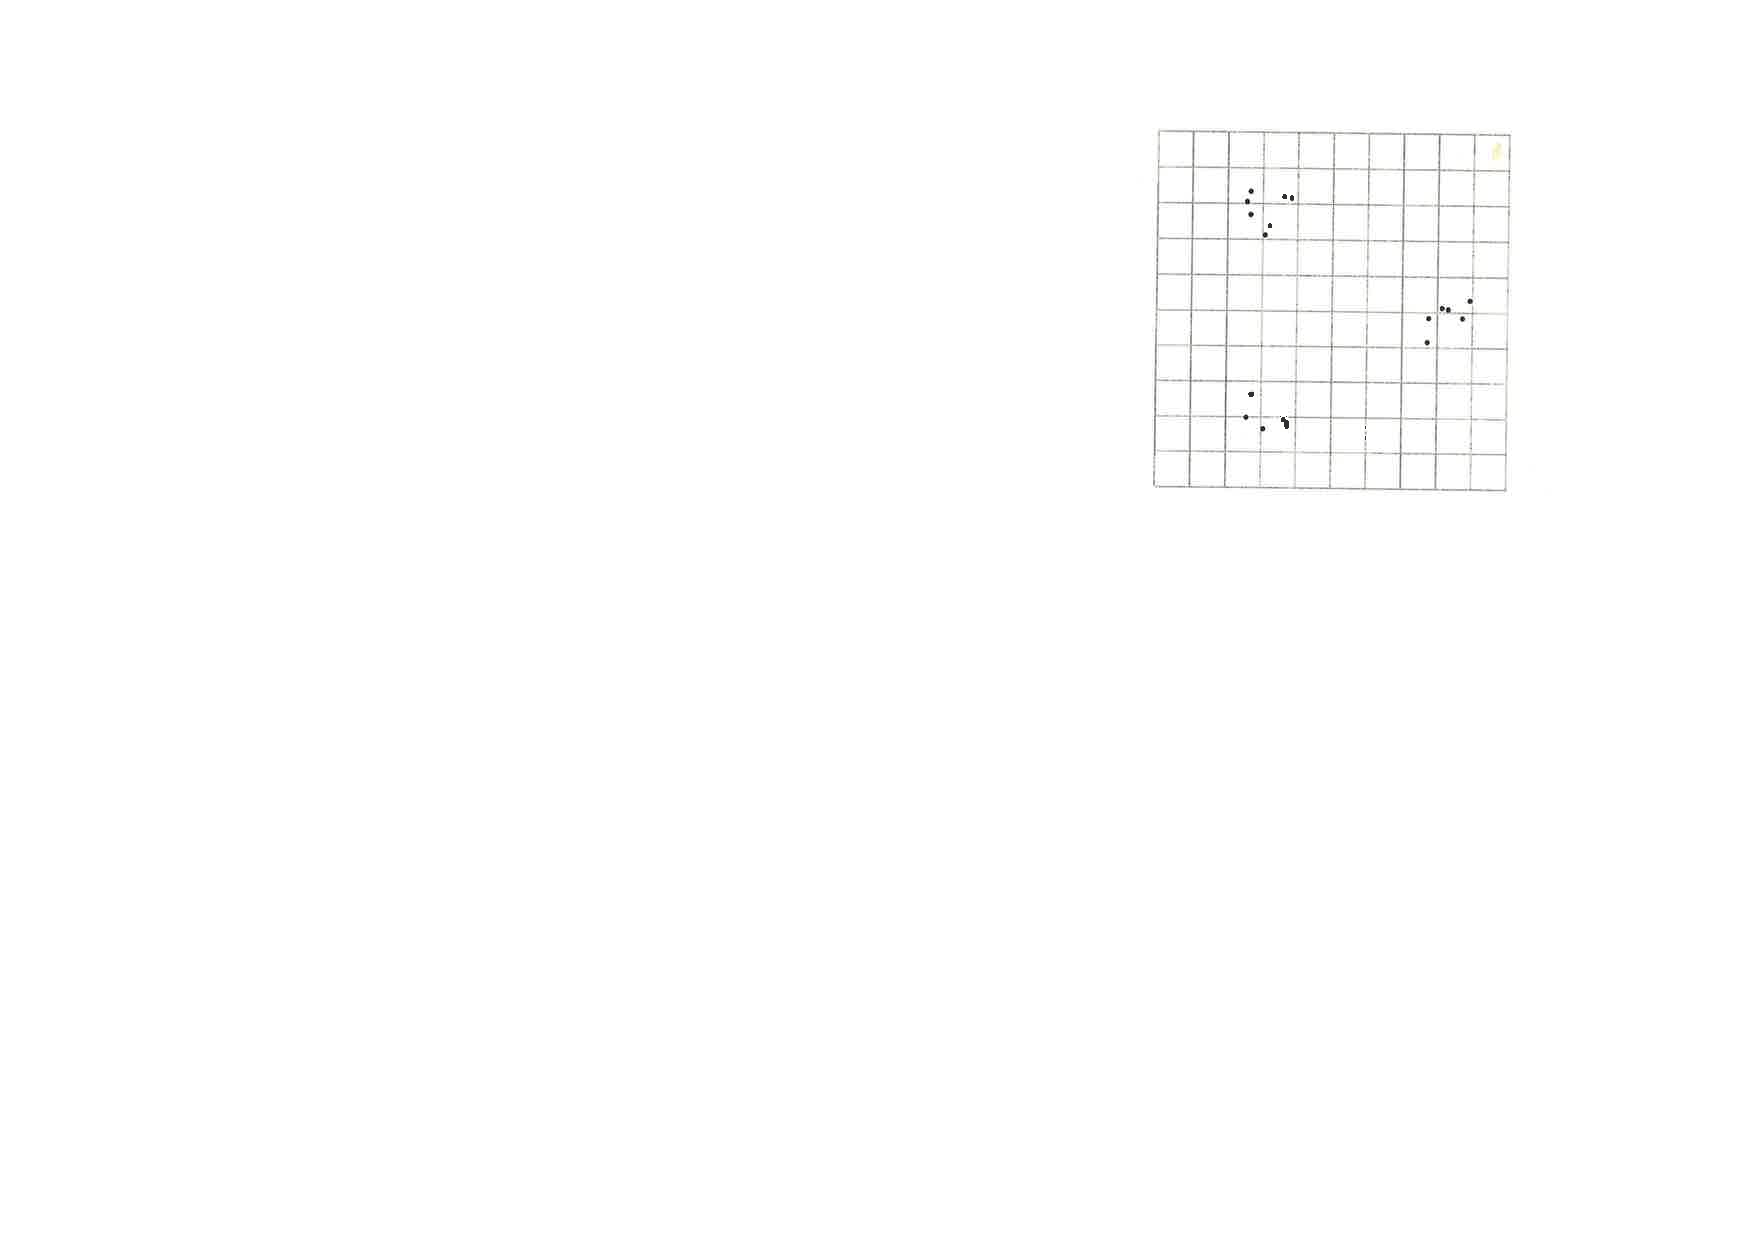
\includegraphics[width=.40
\textwidth]{chap5/figs/fig-agent-distribution}}
\caption{\footnotesize The figure shows the spatial distribution of a set
of 20 agents. There is clustering around three centers.}
\label{figure-agent-distribution}
\end{figure}

In earlier simulations agents were randomly picked
out of the population. 
Now we can base the probability with which two agents interact
on their respective distance and on an
interaction factor, which determines the weight
of the distance. If the interaction factor increases, the
role of distance becomes more important and interactions tend to
reflect the spatial clustering more. Based on this
parameter we can study the evolution of
language when communications between clusters of agents 
increase. 

Initially we let each subgroup evolve towards a shared 
communication. 
Success is never total because there are occasional interactions
with members of other communities, however inner-cluster
communication reaches total success.
However inspection of the agent lexicons reveals that
agents will develop a stable
language within their cluster, but also a
second language, an {\it interlingua}, which is weaker but
shared among the different clusters. This interlingua will
become stronger as more agents interact between clusters.
Thus we observe language diversity due to
the spatial distribution but at the same time the rise 
of an interlingua.

The following vocabularies illustrate this point clearly.
The first vocabulary is taken from an agent from the
leftmost cluster in \figref{figure-agent-distribution}. 
All the words associated with a particular meaning are 
shown together with their score. 
\begin{verbatim}
[M0]: kube[0.88] gutida[0.00] moko[0.00]
[M1]: nugini[0.97] gi[0.83] majiba[0.00]
[M2]: go[0.98] ta[0.00]
[M3]: moma[0.98] ti[0.00] nudo[0.00] kene[0.00]
[M4]: nebu[0.98] me[0.83]
[M5]: tine[0.98]
\end{verbatim}
\begin{verbatim}
[M6]: bo[0.94] babige[0.82]
[M7]: mepabo[0.97] jabeto[0.71] di[0.00]
[M8]: kude[0.90] nado[0.00]
[M9]: pe[0.94] da[0.00]
[M10]: na[0.94] nuguge[0.90] pa[0.80] ne[0.00]
\end{verbatim}
\begin{verbatim}
[M11]: mu[0.98] gite[0.00] paku[0.00]
[M12]: gema[0.96] do[0.33] gapu[0.00]
[M13]: ja[0.67] jo[0.00]
[M14]: dodine[0.88] pibo[0.83] gije[0.00] pupeto[0.00]
[M15]: jiti[0.94] gato[0.64]
\end{verbatim}
\begin{verbatim}
[M16]: bimogu[0.98] ba[0.00]
[M17]: bapi[0.96] ki[0.81] damuti[1,0,0.00]
[M18]: kutume [0.94] bu [0.00] ni[0.00]
[M19]: mugu[0.95] NINU[0.50] pi[0.43] ji[0.00] tu[0.00]
\end{verbatim}
This is the vocabulary for an agent taken from the
rightmost cluster in \figref{figure-agent-distribution}:
\begin{verbatim}
[M0]: gutida[0.79] kube[0.00]
[M1]: gi[0.89] matu[0.85] pumoni[0.00]
[M2]: go[0.95] ta[0.20]
[M3]: kene[0.89] moma[0.82] nudo[0.00] koko[0.00]
[M4]: nebu[0.97] me[0.00] bukugo[0.00]
[M5]: tine[0.90]
\end{verbatim}
\begin{verbatim}
[M6]: babige[0.93] bo[0.00]
[M7]: mepabo[0.90] junipe[0.75] di[0.00]
[M8]: nado[0.96] kude[0.80] puto[0.00]
[M9]: da[0.86] nine[0.71]
[M10]: pa[0.87]
\end{verbatim}
\begin{verbatim}
[M11]: gite[0.88]
[M12]: gema[0.90] gapu[0.87]
[M13]: jo[0.96] ji[0.89] ja[0.00]
[M14]: dodine[0.96] pupeto[0.56] pibo[0.00] gije[0.00]
[M15]: jiti[0.97] gato[0.46]
\end{verbatim}
\begin{verbatim}
[M16]: bimogu[0.97] ba[0.83] pipebe[0.00]
[M17]: ki[0.97] bapi[0.00] ke[,0.00]
[M18]: ni[0.94] kutume[0.80] moko[0.80] mekami[0.00]
[M19]: ninu[0.81] mugu[0.00] pi[0.00]
\end{verbatim}
Some words (for example "tine" for [M5] or "go" for [M2]) are
shared. But generally 
there are at least two words. One word is used preferentially inside the cluster,
the other is known but preferentially used by members of another cluster. Thus
the word "mugu" for [M19] is preferred for the first object in the first
cluster and known but not preferentially used by the agent in the second cluster.
Conversely, "ninu" is preferred for the same meaning by the agent in the second
cluster, although he also knows "mugu".
"mepabo" for [M7] belongs to the interlingua. Both agents
know and use it but they have a strong alternative "jabeto" for 
the first and "junipe" for the second agent. 

\subsection{Language Contact}

When the interaction factor increases, we see further differentiation because\is{language contact}
there is less communication between clusters. When it is decreased, we see more
coherence because there is more intercluster communication. Thus we can
effectively tune divergence or convergence in the simulations
based on the probability of interaction
between communities (clusters) of agents. The effect of 
increased language contact and hence convergence is demonstrated in 
\figref{figure-communicative-success-in-space}. 
The simulation starts from the situation described earlier with three 
clusters of agents that have each evolved a lexicon. 
The interaction between clusters is initially
very weak. At some point (after 4000 games) the intercluster communication is
increased drastically. At first there is a drop in communicative
success but then total communicative success is again reached.

\begin{figure}[htbp]
  \centerline{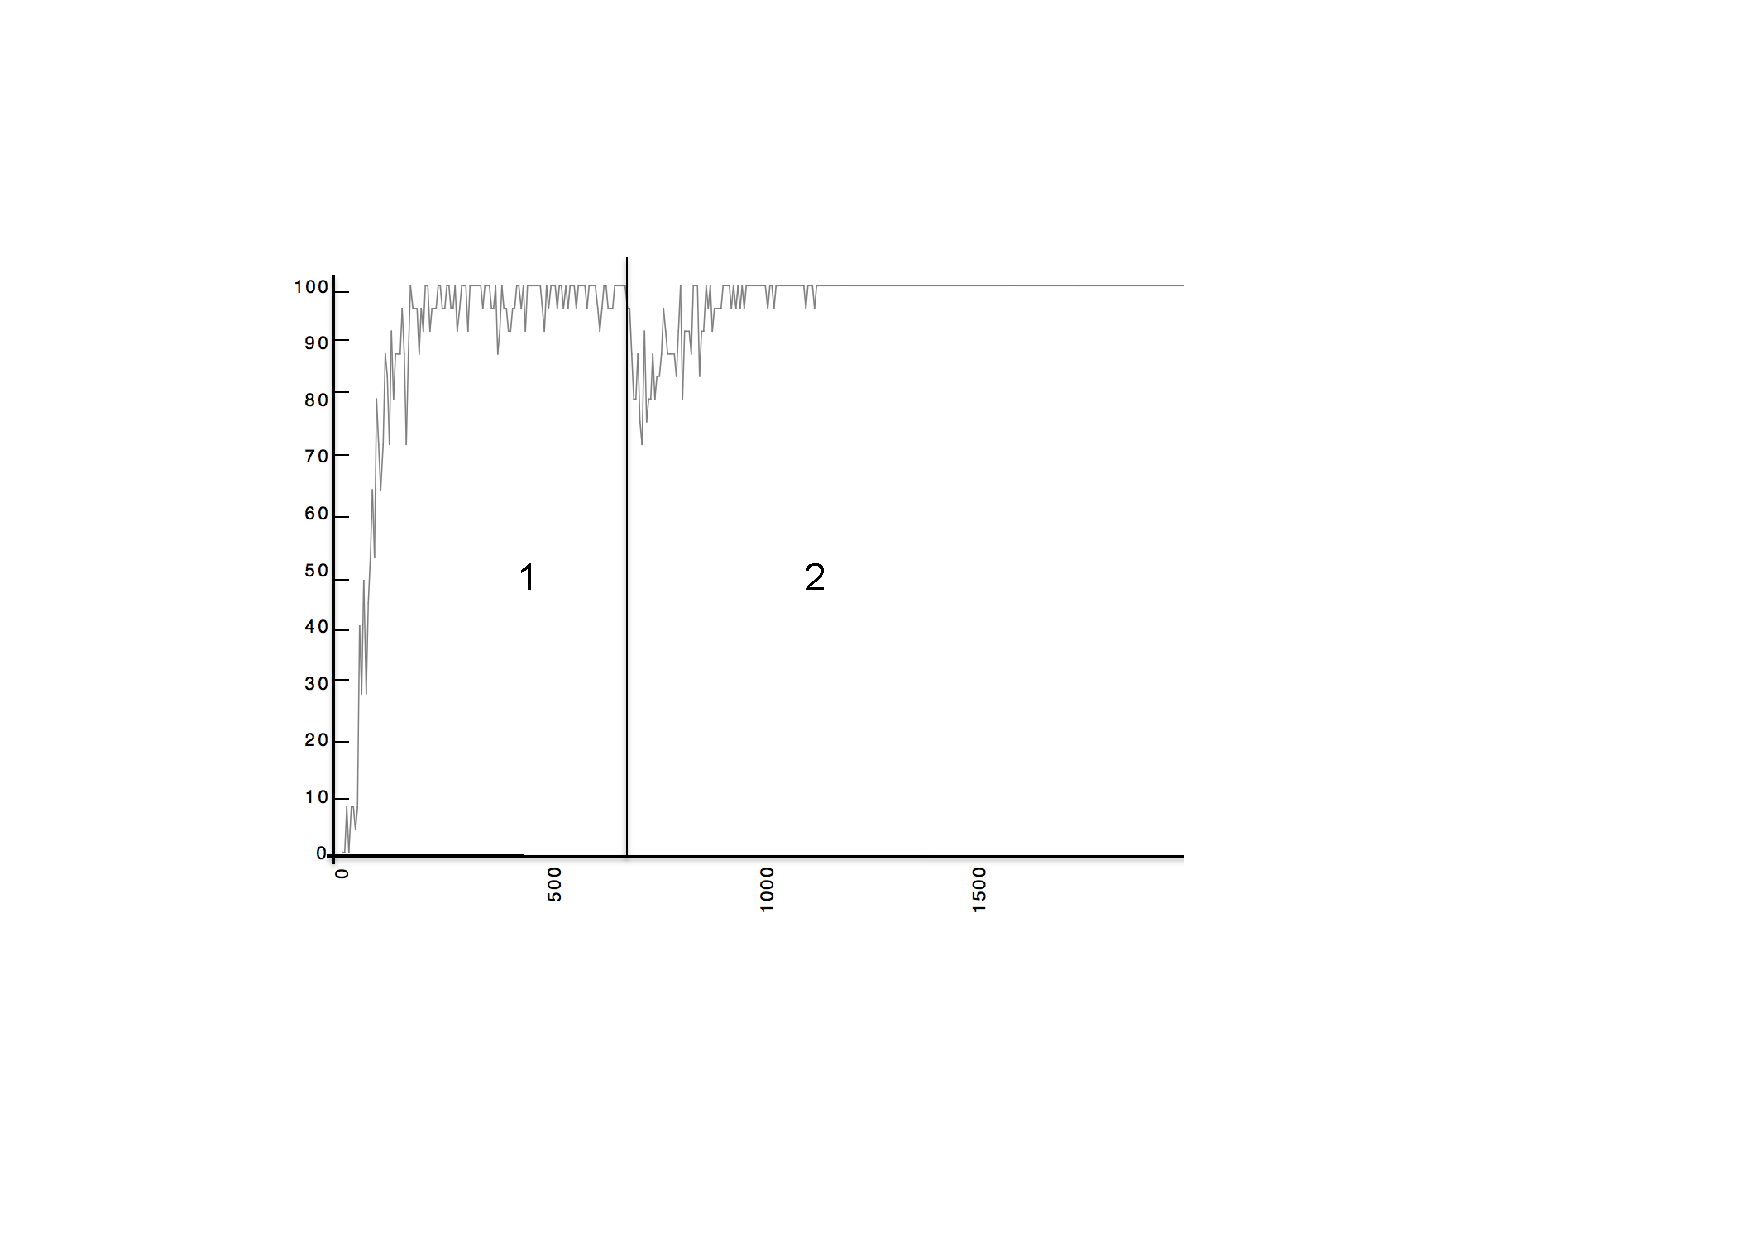
\includegraphics[width=.65\textwidth]{chap5/figs/comm-succ}}
\caption{\footnotesize Evolution of average communicative success per 25 games
in a group of agents with first weak (phase 1) and then strong
interactions (phase 2).}
\label{figure-communicative-success-in-space}
\end{figure}

However, this general evolution hides the more interesting
developments. \figref{figure-coherence-in-space}
shows the evolution of coherence for each
cluster (a, b, c) separately and
also for the total set of agents. As long as the agents
have relatively little contact, total coherence is low
although the lexical coherence within each cluster is high. 
Total coherence starts to increase with increased contact. Coherence in
each cluster diminishes somewhat because the agents in the
cluster are in the process of accomodating to the global lexicon. 
This means that the
languages of the different groups are in the process of
merging due to the increased language contact.

\begin{figure}[htbp]
  \centerline{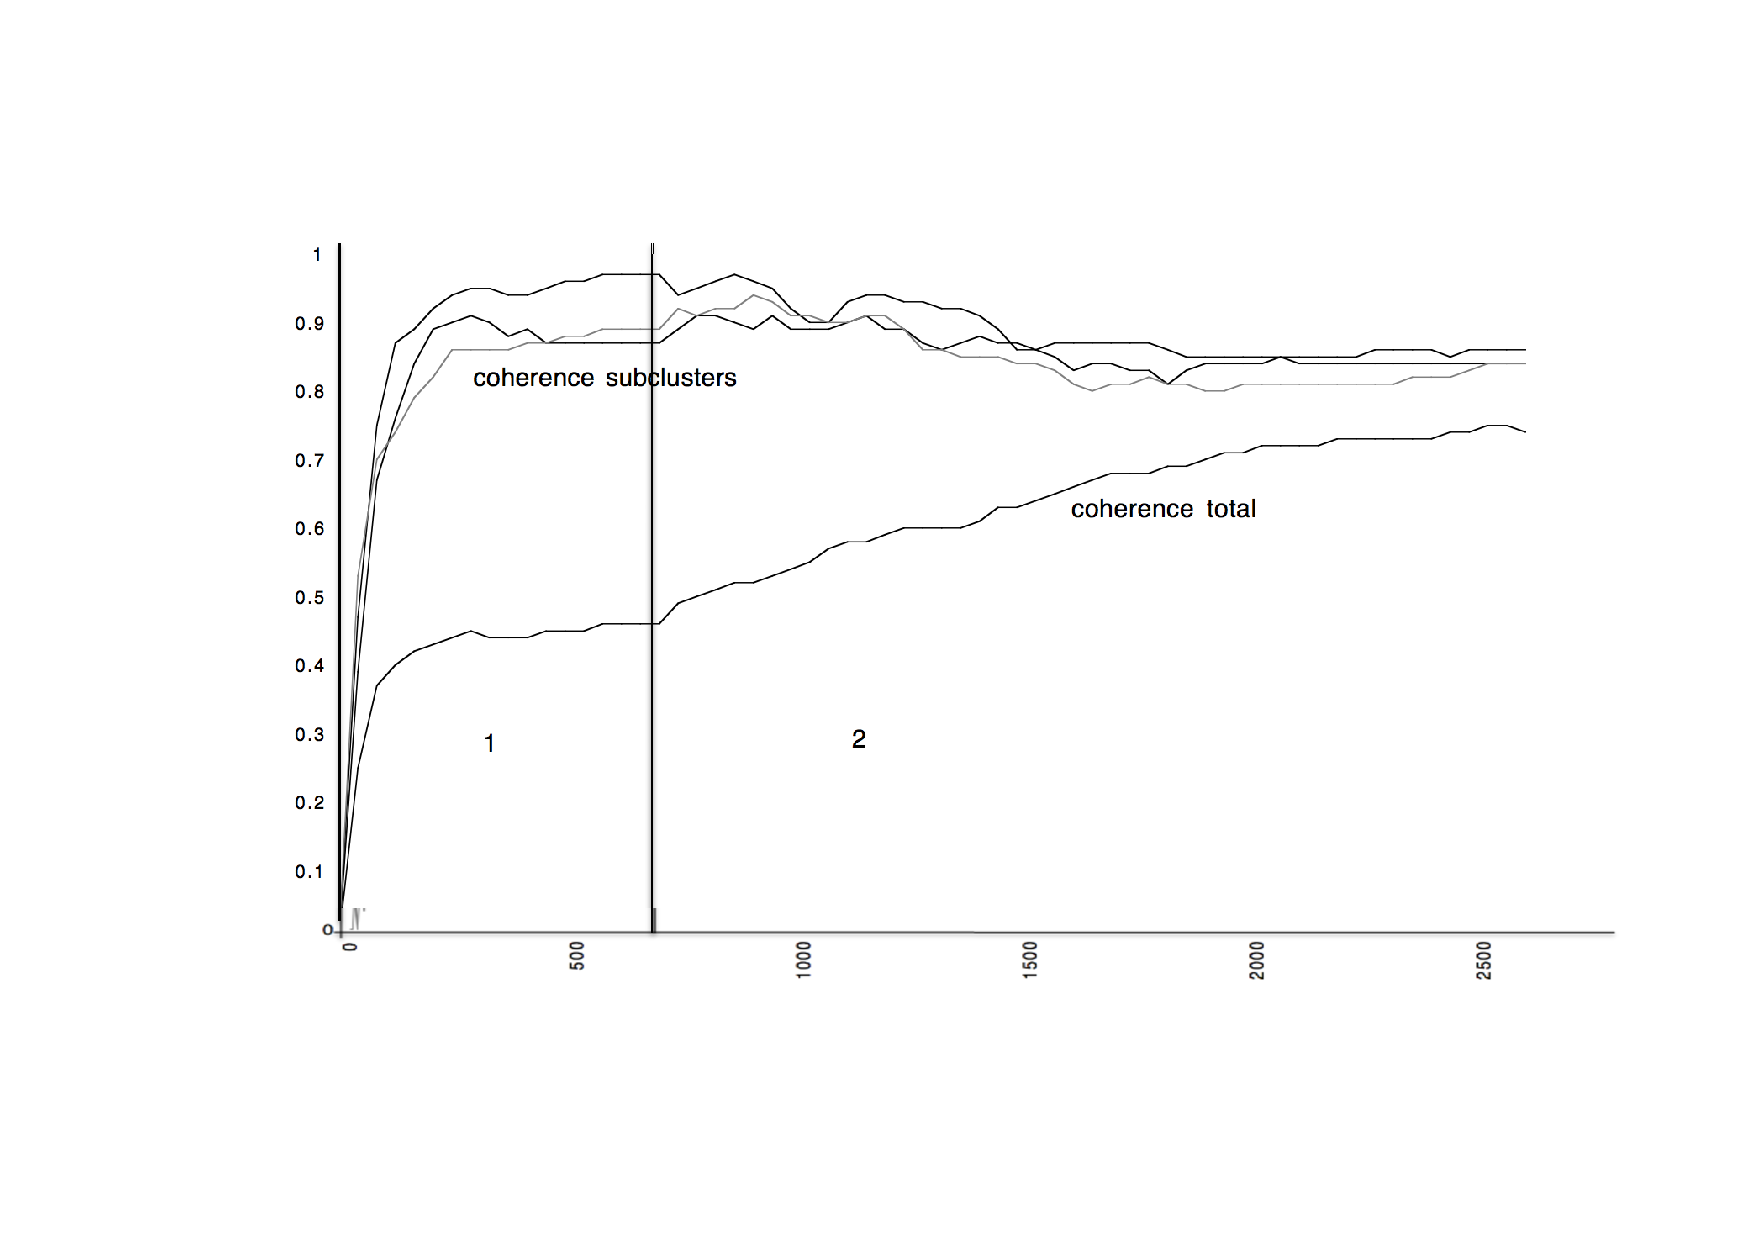
\includegraphics[width=.80\textwidth]{chap5/figs/coherence}}
\caption{Evolution of coherence in the total population 
and in the individual clusters is shown on the same
scale as the previous figure. When contact 
is increased (phase 2), global coherence begins to rise steadily.}
\label{figure-coherence-in-space}
\end{figure}
Simulations show that, just as in human languages,
increased contact causes at first a rapid increase in
bilingualism, then a gradual mixing of the languages, and, 
if the contact
continues, an evolution towards complete coherence. 
The more rapid the contact is
increased, the faster the three phases can be observed. 

\section{Conclusions}

A population of agents following a simple set of 
behavior rules and using an associative memory
can give rise to a shared repertoire of form-meaning 
associations, giving the agents a total average success in 
communication. Once a shared repertoire comes
into existence, it locks into an equilibrium state and 
gets transmitted from one generation to the next in a 
cultural process, as long as the rate of population change 
is not too high. The population can also cope with 
an in- and outflux of meanings, in the sense that 
the lexicon constracts or expands in relation to the 
demands from an evolving set of possible meanings.  

The mechanisms I have proposed here for the Naming Game are
remarkable in many ways. It clearly shows that a
shared set of conventions
can arise without an omniscient central co-ordinator and
without any prior knowledge of the lexicon built into 
the agents. The Naming Game also demonstrates
a new way to model and thus
investigate linguistic phenomena. Existing formal models
of language, such as generative grammars, only model static
competence of a single idealised speaker in a homogeneous language
community. Using the framework of language games 
played by populations of agents, we can model the 
emergence and evolution of language in an inhomogeneous community
and study language use as well as change 
through language contact. 

The Naming Game is a minimal model of communication 
between agents and far removed from the full complexity 
of human natural language. Moreover we made a number of 
simplifying assumptions, thus putting up scaffolds to
construct this initial model. The most important assumption
was that the meaning of a word can be unambiguously 
known by the speaker and hearer independently of language. 
This assumption is of course not valid for human 
beings, and neither is it valid for the Talking Heads. 



